\documentclass{libs/XJTLU_format}

%\documentclass{article}

%%%%%%%%%%%%%%%%%%%%%%%%%%%%%%%%%%%%%%%%%%%%%%%%%%%%%%%%%%%%%%%%%%%%%%%%%%%%%%
% \embedvideo{<poster or text>}{<video file (MP4+H264)>}
%%%%%%%%%%%%%%%%%%%%%%%%%%%%%%%%%%%%%%%%%%%%%%%%%%%%%%%%%%%%%%%%%%%%%%%%%%%%%%
\usepackage[bigfiles]{pdfbase}
\usepackage{amssymb}
\usepackage{booktabs}
\usepackage[version=4]{mhchem}

\ExplSyntaxOn
%%begin novalidate
\cs_new:Npn\embedvideo#1#2{
%%end novalidate
  \leavevmode
  \pbs_pdfobj:nnn{}{fstream}{{}{#2}}
  \pbs_pdfobj:nnn{}{dict}{
    /Type/Filespec/F~(#2)/UF~(#2)
    /EF~<</F~\pbs_pdflastobj:>>
  }
  \tl_set:Nx\video{\pbs_pdflastobj:}%
  %
  \pbs_pdfobj:nnn{}{dict}{
    /Type/RichMediaInstance/Subtype/Video
    /Asset~\video
    /Params~<</Binding/Foreground>>
  }
  %
  \pbs_pdfobj:nnn{}{dict}{
    /Type/RichMediaConfiguration/Subtype/Video
    /Instances~[\pbs_pdflastobj:]
  }
  %
  \pbs_pdfobj:nnn{}{dict}{
    /Type/RichMediaContent
    /Assets~<<
      /Names~[(#2)~\video]
    >>
    /Configurations~[\pbs_pdflastobj:]
  }
  \tl_set:Nx\rmcontent{\pbs_pdflastobj:}%
  %
  \pbs_pdfobj:nnn{}{dict}{
    /Activation~<<
      /Condition/XA
      /Presentation~<<
        /Transparent~true
        /Style/Embedded
        /PassContextClick~true
      >>
    >>
    /Deactivation~<</Condition/PC>>
  }
  %
  \hbox_set:Nn\l_tmpa_box{#1}
  \tl_set:Nx\l_box_wd_tl{\dim_use:N\box_wd:N\l_tmpa_box}
  \tl_set:Nx\l_box_ht_tl{\dim_use:N\box_ht:N\l_tmpa_box}
  \tl_set:Nx\l_box_dp_tl{\dim_use:N\box_dp:N\l_tmpa_box}
  \pbs_pdfxform:nnnnn{1}{1}{}{}{\l_tmpa_box}
  %
  \pbs_pdfannot:nnnn{\l_box_wd_tl}{\l_box_ht_tl}{\l_box_dp_tl}{
    /Subtype/RichMedia
    /BS~<</W~0/S/S>>
    /Contents~(embedded~video~file:#2)
    /NM~(rma:#2)
    /AP~<</N~\pbs_pdflastxform:>>
    /RichMediaSettings~\pbs_pdflastobj:
    /RichMediaContent~\rmcontent
  }
  \phantom{#1}
}%
\ExplSyntaxOff
%%%%%%%%%%%%%%%%%%%%%%%%%%%%%%%%%%%%%%%%%%%%%%%%%%%%%%%%%%%%%%%%%%%%%%%%%%%%%%


% % Inserting the preamble file with the packages
% %%%%%%%%%%%%%%%%%%%%%%%%%%%%%%%%%%%%%%%%%%%%%%%%%%%%%%%%%%%%%%%%%%%%%
%% This file contains the packages that can be used in the beamer. %%
%%%%%%%%%%%%%%%%%%%%%%%%%%%%%%%%%%%%%%%%%%%%%%%%%%%%%%%%%%%%%%%%%%%%%
% Package to fonts family
\usepackage[T1]{fontenc}
% Package to accentuation
\usepackage[utf8]{inputenc}
% Package to Figures
\usepackage{graphicx}
% Package to the colors
\usepackage{color}
% Package to the colors
\usepackage{xcolor}
% Packages to math symbols and expressions
\usepackage{amsfonts, amssymb, amsmath}
% Package to multiple lines and columns in table
\usepackage{multirow, array} 
% Package to create pseudo-code
% For more detail of this package: http://linorg.usp.br/CTAN/macros/latex/contrib/algorithm2e/doc/algorithm2e.pdf
\usepackage{algorithm2e}
% Package to insert code
\usepackage{listings} 
\usepackage{keyval}
% Package to justify text
\usepackage[document]{ragged2e}
% Package to manage the bibliography
\usepackage[backend=biber, style=numeric, sorting=none]{biblatex}
% Package to facilities quotations
\usepackage{csquotes}
% Package to use multicols
\usepackage{multicol}
\usepackage{transparent}

% % Inserting the references file
% \bibliography{references.bib}

% % Title
% \title[MAT 214_Processing and Properties of Ceramic Materials]{\textbf{MAT 214: Processing and Properties of Ceramic Materials}}
% % Subtitle
% \subtitle{Introduction to Ceramic Materials}
% % Author of the presentation
% \author{Prof. Joshua C. Agar}
% % Institute's Name
% \institute[Lehigh University]{
%     % email for contact
%     \normalsize{\email{jca318@lehigh.edu}}
%     \newline
%     % Department Name
%     \department{Materials Science and Engineering}
%     \newline
%     % University name
%     \university{Lehigh Univeristy}
% }
% % date of the presentation
% \date{\today}

% %\newcommand*{\keys}{\fontfamily{cmtt}\selectfont}

%%%%%%%%%%%%%%%%%%%%%%%%%%%%%%%%%%%%%%%%%%%%%%%%%%%%%%%%%%%%%%%%%%%%%%%%%%%%%%


% Inserting the preamble file with the packages
%%%%%%%%%%%%%%%%%%%%%%%%%%%%%%%%%%%%%%%%%%%%%%%%%%%%%%%%%%%%%%%%%%%%%
%% This file contains the packages that can be used in the beamer. %%
%%%%%%%%%%%%%%%%%%%%%%%%%%%%%%%%%%%%%%%%%%%%%%%%%%%%%%%%%%%%%%%%%%%%%
% Package to fonts family
\usepackage[T1]{fontenc}
% Package to accentuation
\usepackage[utf8]{inputenc}
% Package to Figures
\usepackage{graphicx}
% Package to the colors
\usepackage{color}
% Package to the colors
\usepackage{xcolor}
% Packages to math symbols and expressions
\usepackage{amsfonts, amssymb, amsmath}
% Package to multiple lines and columns in table
\usepackage{multirow, array} 
% Package to create pseudo-code
% For more detail of this package: http://linorg.usp.br/CTAN/macros/latex/contrib/algorithm2e/doc/algorithm2e.pdf
\usepackage{algorithm2e}
% Package to insert code
\usepackage{listings} 
\usepackage{keyval}
% Package to justify text
\usepackage[document]{ragged2e}
% Package to manage the bibliography
\usepackage[backend=biber, style=numeric, sorting=none]{biblatex}
% Package to facilities quotations
\usepackage{csquotes}
% Package to use multicols
\usepackage{multicol}
\usepackage{transparent}

% Inserting the references file
\bibliography{references.bib}

% Title
\title[MAT 214 Spring 2022]{\textbf{MAT 214:  Processing and Properties of Ceramic Materials}}
% Subtitle
\subtitle{Crystal Structures in Ceramics}
% Author of the presentation
\author{Prof. Joshua C. Agar}
% Institute's Name
\institute[Lehigh University]{
    % email for contact
    \normalsize{\email{jca318@lehigh.edu}}
    \newline
    % Department Name
    \department{Materials Science and Engineering}
    \newline
    % University name
    \university{Lehigh Univeristy}
}
% date of the presentation
\date{\today}

%%%%%%%%%%%%%%%%%%%%%%%%%%%%%%%%%%%%%%%%%%%%%%%%%%%%%%%%%%%%%%%%%%%%%%%%%%%%%%%%%%
%% Start Document of the Presentation                                           %%               
%%%%%%%%%%%%%%%%%%%%%%%%%%%%%%%%%%%%%%%%%%%%%%%%%%%%%%%%%%%%%%%%%%%%%%%%%%%%%%%%%%
\begin{document}

% insert the code style
%%%%%%%%%%%%%%%%%%%%%%%%%%%%%%%%%%%%%%%%%%%%%%%%%%%%%%%%%%%%%%%%%%%%%%%%%%%%%%%%%%%
%% This file contains the style of the codes show in slides.                     %%
%% The package used is listings, but it possible to used others.                 %%
%%%%%%%%%%%%%%%%%%%%%%%%%%%%%%%%%%%%%%%%%%%%%%%%%%%%%%%%%%%%%%%%%%%%%%%%%%%%%%%%%%%

% color used in the code style
\definecolor{codegreen}{rgb}{0,0.6,0}
\definecolor{codegray}{rgb}{0.5,0.5,0.5}
\definecolor{codepurple}{rgb}{0.58,0,0.82}
\definecolor{codebackground}{rgb}{0.95,0.95,0.92}

% style of the code!
\lstdefinestyle{codestyle}{
    backgroundcolor=\color{codebackground},   
    commentstyle=\color{codegreen},
    keywordstyle=\color{magenta},
    numberstyle=\tiny\color{codegray},
    stringstyle=\color{codepurple},
    basicstyle=\ttfamily\footnotesize,
    frame=single,
    breakatwhitespace=false,         
    breaklines=true,                 
    captionpos=b,                    
    keepspaces=true,                 
    numbers=left,                    
    numbersep=5pt,                  
    showspaces=false,                
    showstringspaces=false,
    showtabs=false,                  
    tabsize=2,
    title=\lstname 
}

\lstset{style=codestyle}


%% ---------------------------------------------------------------------------
% First frame (with tile, subtitle, ...)
\begin{frame}{}
    \maketitle
\end{frame}

\section{Learning Objectives}
\begin{frame}{Learning Objectives}
\begin{itemize}
    \item An understanding of how the nature of the atomic constituents influence the resulting crystallographic structures
    \pause
    \item A understanding of some of the ways crystal structure can influence properties
    \pause
    \item An understanding of the relative energetics of different crystallographic configurations
    \pause
    \item A working knowledge of Pauling's Rules
    \pause
    \item An understanding of common binary ceramic crystal structures
    \pause
    \item An understanding of common ternary ceramic crystal structures
    \pause
    \item An appreciation for the complexity of ceramic crystal structures.
\end{itemize}
    
\end{frame}

\section{Ceramic Crystals}
\begin{frame}{Ceramic Bonding}

\centering
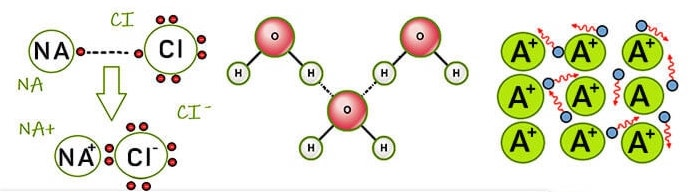
\includegraphics[height=1in]{Silde_Template/images/Ionic-vs-Covalent-vs-Metallic-bonds.jpeg}

    \begin{itemize}
        \item In the past (MAT 033) we have primarily considered crystal structures formed by metallic or ionic bonds $\rightarrow$ Ceramics are much more complicated. \pause
        \item Ceramics tend to have mixed covalent ionic character\pause
    \end{itemize}\\

    \justifying
    Rules: 
    \begin{itemize}
        \item Two atoms with similar electronegativity will form metallic or covalent bonds \pause
        \item Two atoms with different electronegativity will be partially ionic \pause
    \end{itemize}
\end{frame}

\begin{frame}{Fraction of Ionic Character}
The fraction of ionic character differs with the electronegativity of the two atoms\\[0.3em]
\centering
$\% ionic = 1-\exp[-0.25(X_m - X_x)^2]$
\pause

\begin{columns}{\textwidth}
      \begin{column}{0.5\textwidth}
      \centering
      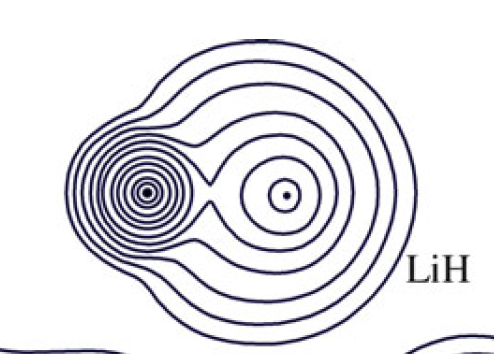
\includegraphics[height=1in]{Silde_Template/images/Screen Shot 2022-01-19 at 12.08.22 PM.png}
      \end{column}
      \begin{column}{0.5\textwidth}
          \centering
          
\includegraphics[height=1in]{Silde_Template/images/Screen Shot 2022-01-19 at 12.08.32 PM.png}
      \end{column}
  \end{columns}
\end{frame}

\begin{frame}{Terms and Definitions: Crystal lattice}
\textbf{Crystal lattice:} A three-dimensional array of points related by translational symmetry. 
\pause
\begin{itemize}
    \item We can fully describe such a lattice by
three vectors \textbf{a}, \textbf{b}, \textbf{c}, and three angles, $\alpha$, $\beta$, $\gamma$.
\end{itemize}
\pause
\centering         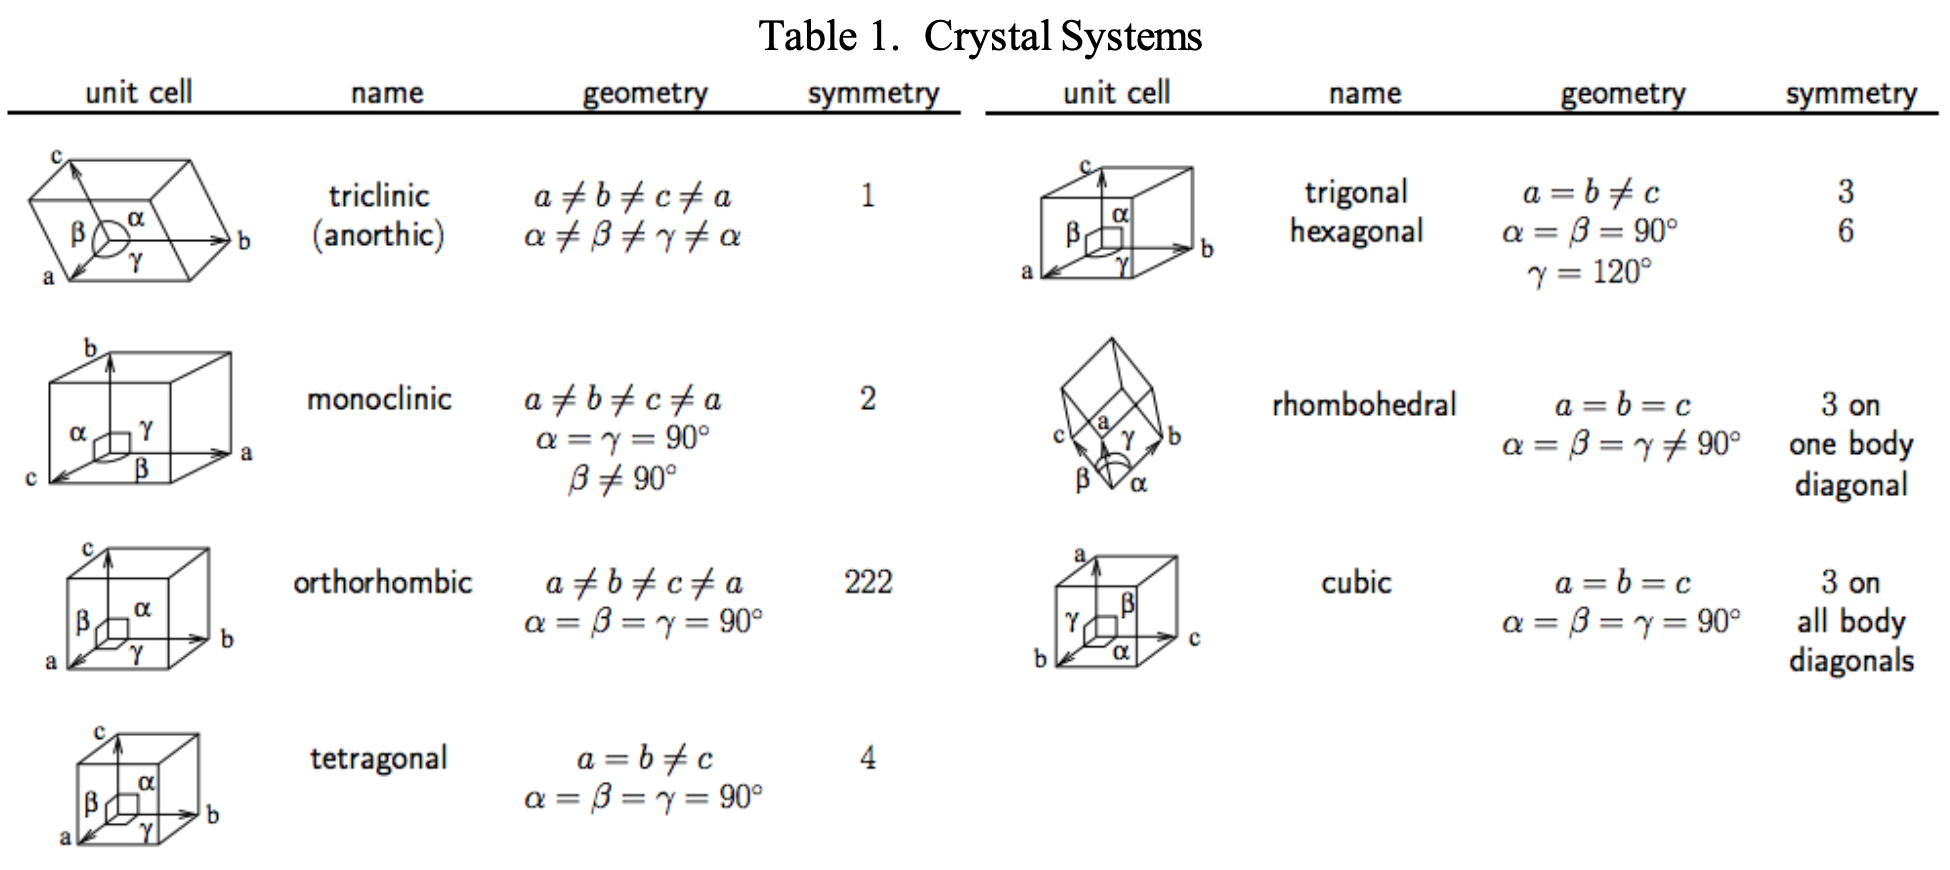
\includegraphics[height=2in]{Silde_Template/images/7_crystal_systems.png}

\end{frame}

\begin{frame}{Terms and Definitions: Basis}
Group of atoms associated with each and every lattice point. \\[1em]
\centering
\textbf{Bravais Lattice = Basis + Crystal Structure}
\centering
\pause
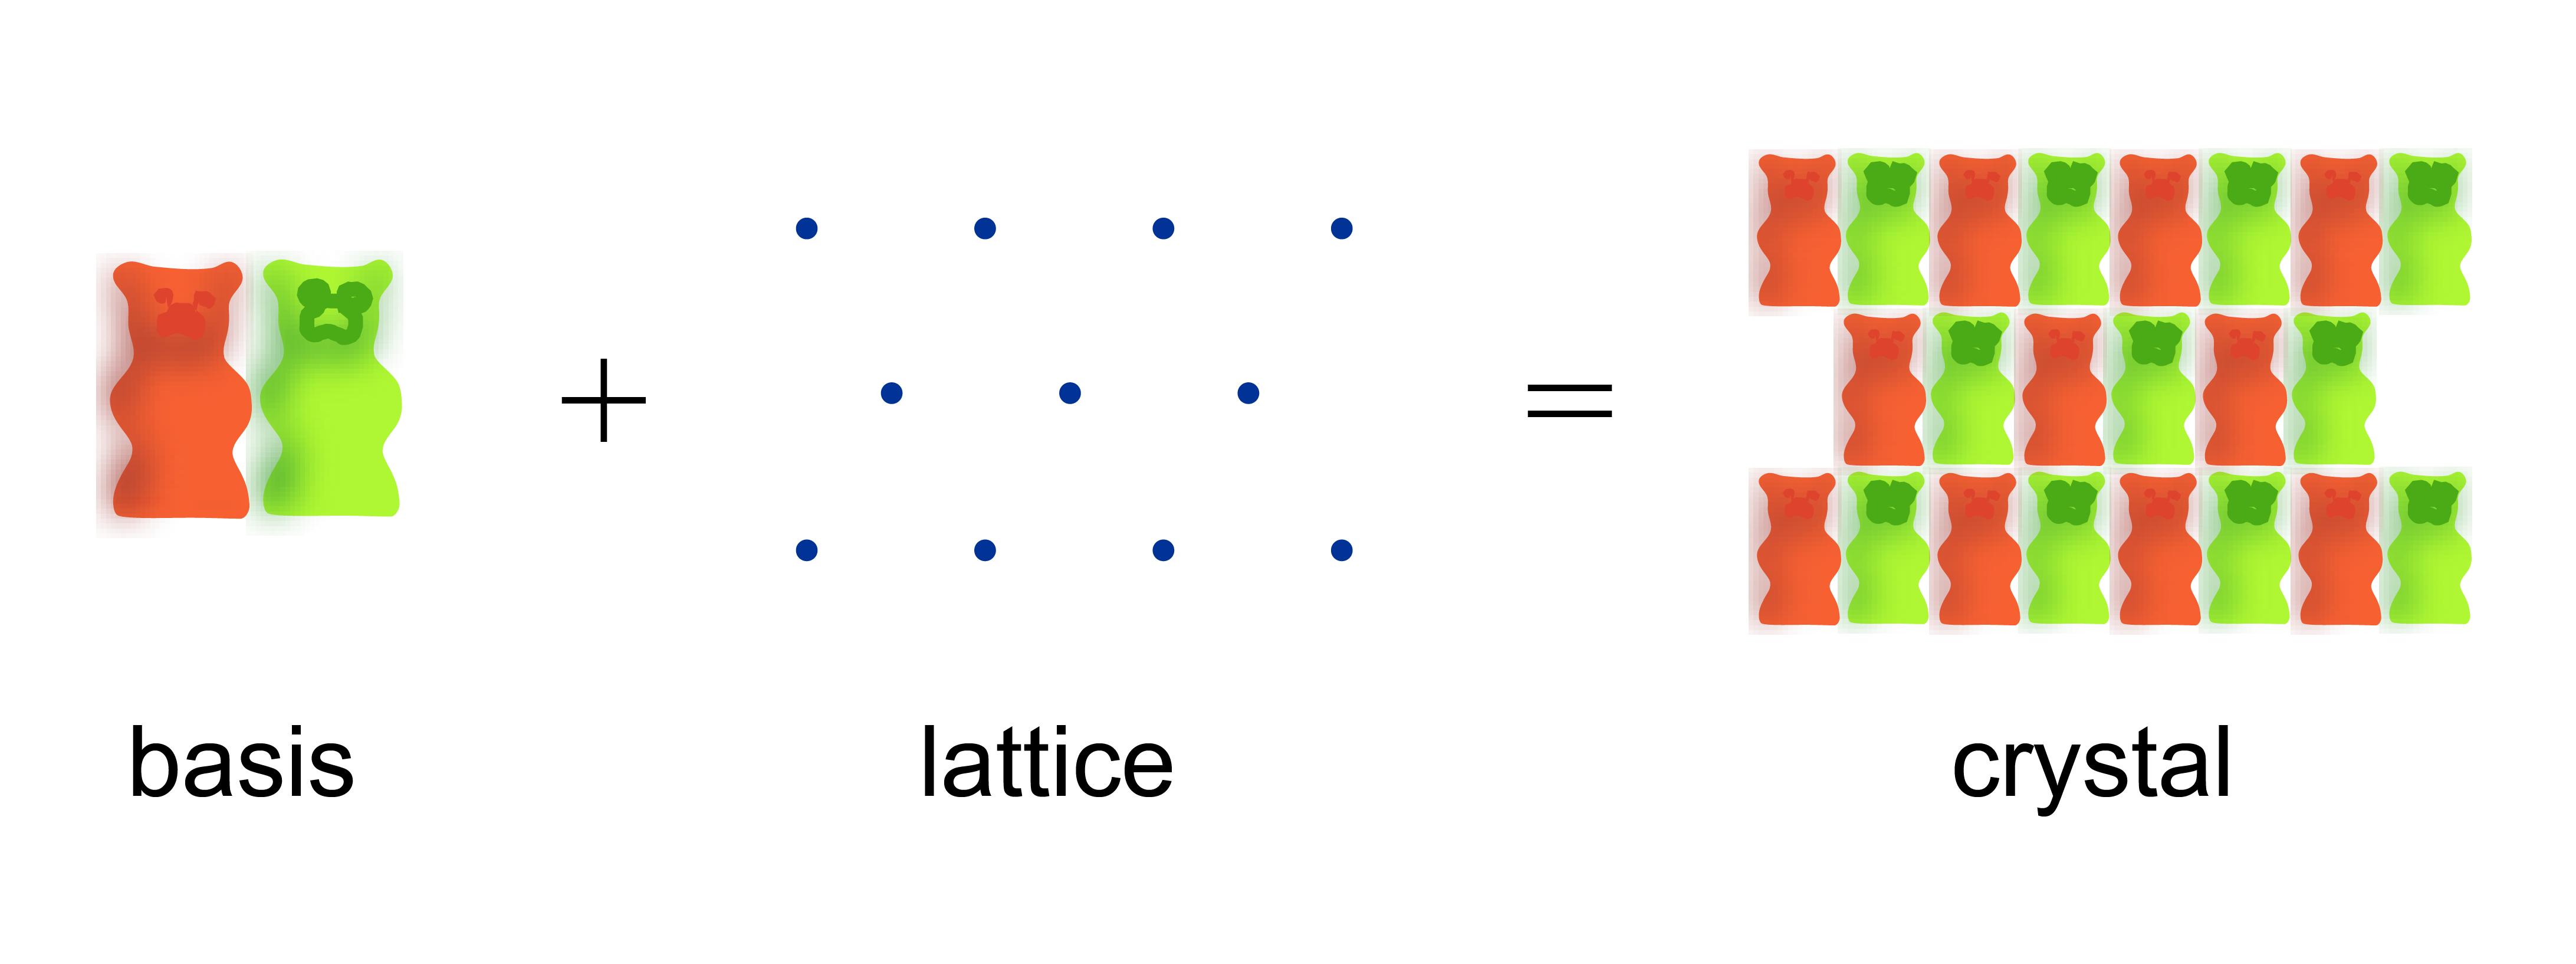
\includegraphics[height=1in]{Silde_Template/images/basis-lattice-crystal-01.png}
\end{frame}

\begin{frame}{Terms and Definitions: Bravais lattice}
    Within each crystal lattice there are 14 different ways to arrange lattice points. \pause
    \begin{itemize}
        \item Primitive (P) lattices—one lattice point per unit cell
        \item Body-centered (I) lattices—a lattice point at the corners and one in the center of the cell
        \item A-, B-, C- or F-centered lattices—a lattice point at the corners and others at one (A, B, C) or all three (F) of the faces
    \end{itemize}
\end{frame}

\begin{frame}{Terms and Definitions: Bravais lattice}
    \centering
    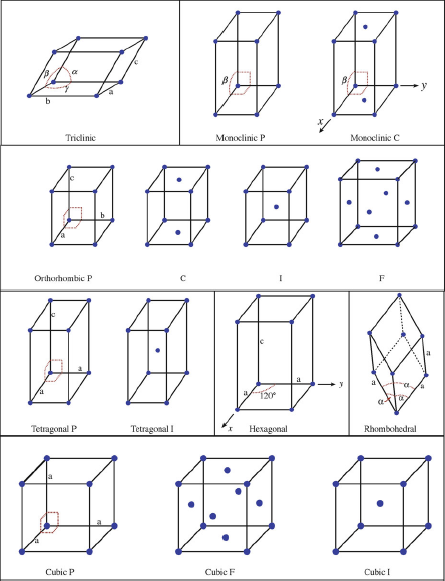
\includegraphics[height=3in]{Silde_Template/images/Bravais_lattice.png}
\end{frame}

\begin{frame}{Coordination Number}
\textbf{Coordination number (CN):} Number of nearest neighbors.\\[1em]

\centering
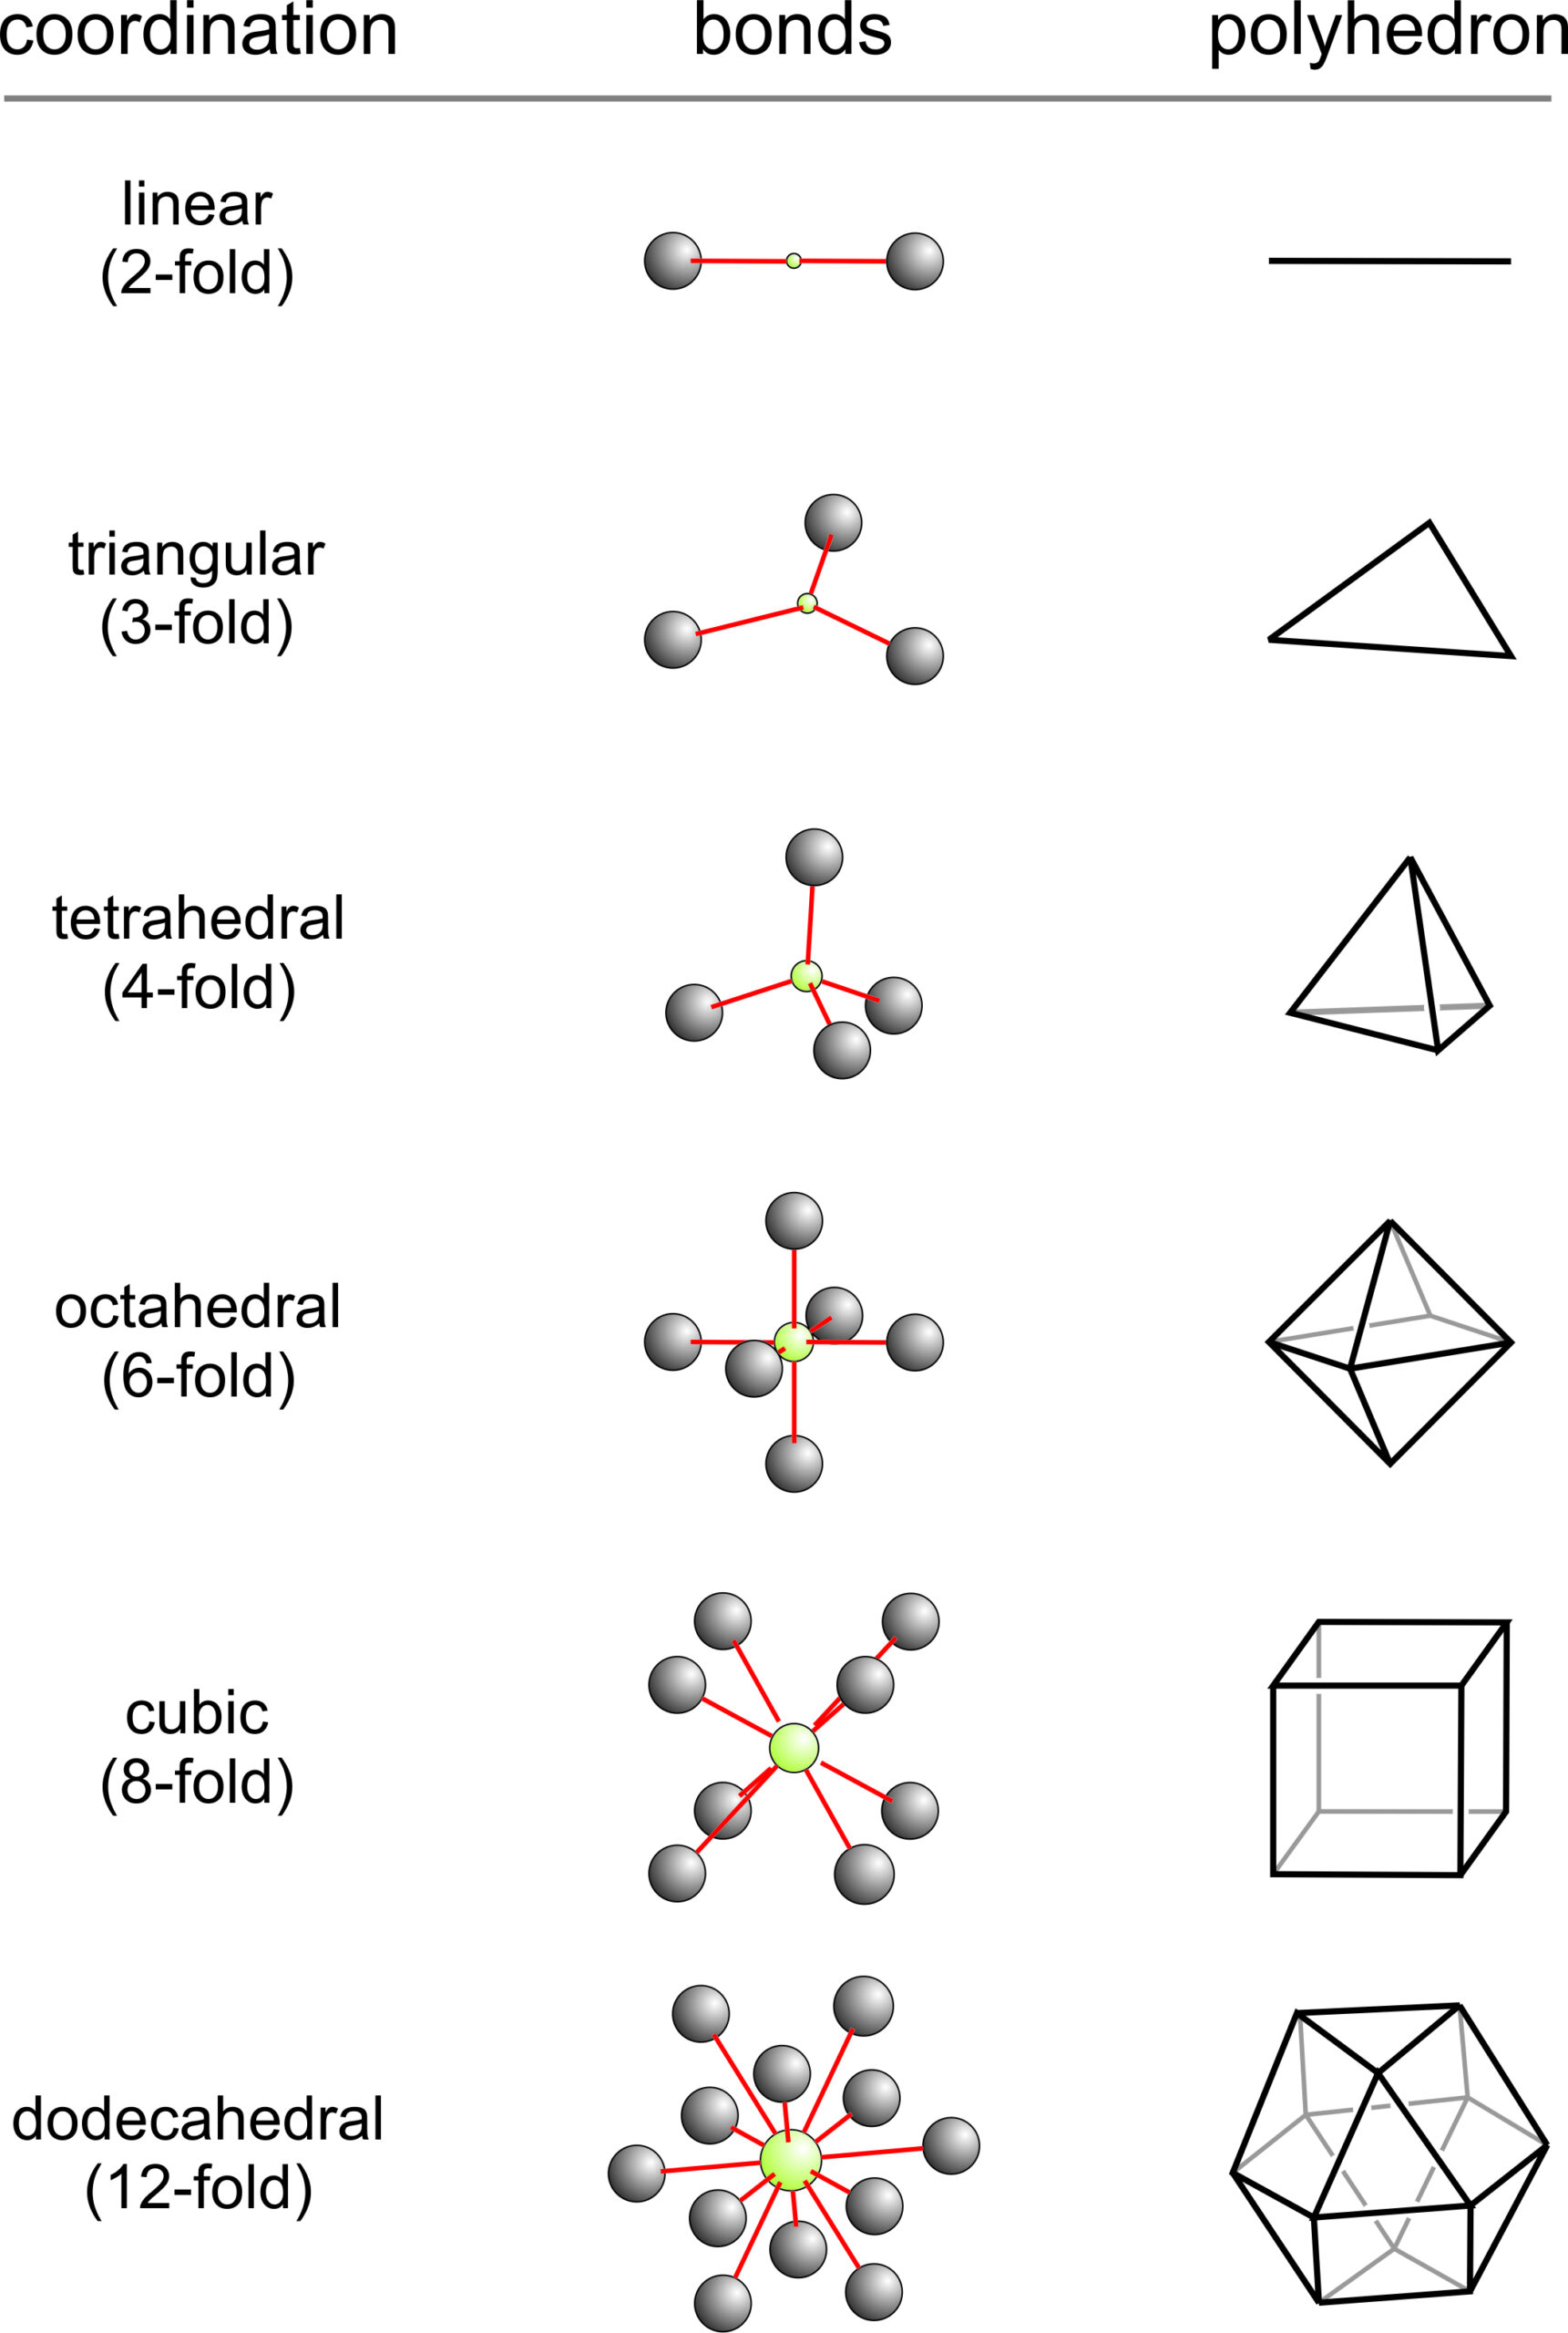
\includegraphics[height=2.5in]{Silde_Template/images/different-coordinations-v4-1-scaled.jpg}
\end{frame}

\begin{frame}{Why do we care so much about crystallography?}
All properties are based on the underlying crystallography \pause

\begin{itemize}
    \item \textbf{Diffusion:} Depends on size and number of interstitial sites \pause
    \item \textbf{Deformation by slip or twinning:}  The slip direction is usually along a close-packed direction. The slip plane is usually a closely packed plane or one that does not put like charges in juxtaposition. 
    \pause
    \item \textbf{Piezoelectricity:} Crystals must be noncentrosymmetric
    \pause
    \item \textbf{Thermal conductivity:} Electrical and phonon conductivity is directly determined by the underlying crystal structure
    \pause
    \item \textbf{Fracture:} Often crystallographic but not always (e.g., glass and cubic zirconia)
    \pause
    \item \textbf{Cleavage:} Always crystallographic. Cleavage planes have high atomic density, but we also need to consider charge.
    \pause
    \item \textbf{Ferrimagnetism:} In ferrimagnets the coordination number of the magnetic cation (usually a Fe ion) determines its behavior in an applied magnetic field.
\end{itemize}
\end{frame}

\section{Pauling's Rules}
\begin{frame}{Pauling's Rule 1}
    \textbf{Rule 1:} A coordinated polyhedron of anions is formed about each cation. The cation–anion distance is determined by the sum of the two radii, and the CN is determined by the radius ratio:\\[1em]
    
    \centering
    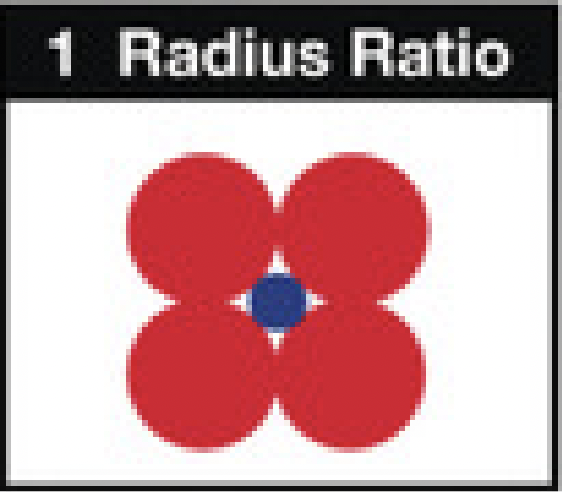
\includegraphics[height=1in]{Silde_Template/images/1.png}
    
    $\textrm{Radius Ratio} = \frac{r_c}{r_a}$
    \pause
    \begin{itemize}
        \item Cation (+ charged) are always smaller than anions (- charged)
    \end{itemize}\\[1em]
    
    \pause
    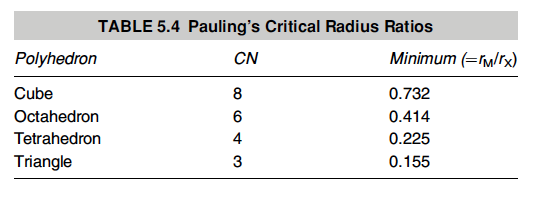
\includegraphics[height=1in]{Silde_Template/images/Paulings_Rules.png}

\end{frame}

\begin{frame}{Pauling's Rule 2}
    \textbf{Rule 2:} In a stable structure, the total electrostatic strength of the bonds, S, reaching an anion in a coordination polyhedron from all neighboring cations should be equal to the charge of the anion.\\[1em]
    \pause
    
    \centering
    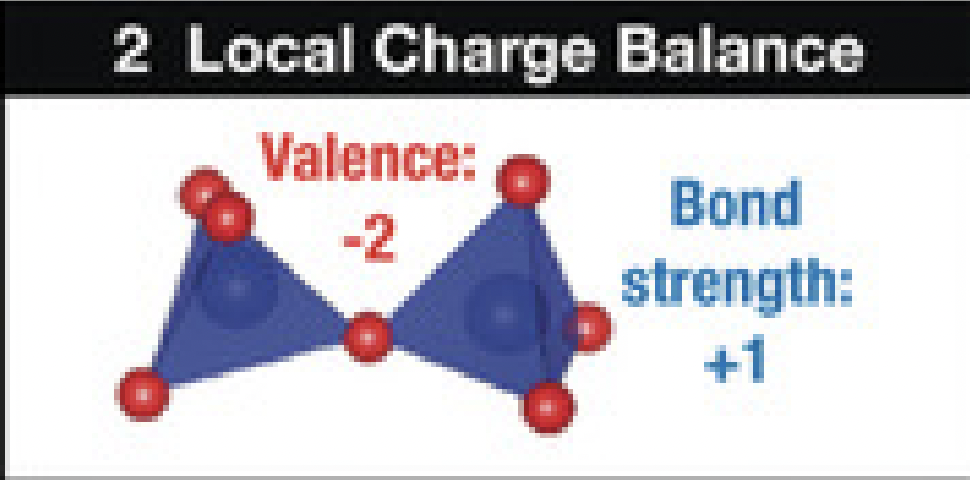
\includegraphics[height=1in]{Silde_Template/images/2.png}
    
    \pause
    \centering
    $S = \frac{Z_c}{CN}$
    \\[1em]
    
    \justifying
    $Z_c$ - is the charge of the cation\\
    $CN$ - is the coordination number\\[1em]
    \pause
    A stable ionic structure is arranged to preserve local \emph{electroneutrality}, so that the sum of the strengths of the electrostatic bonds to an anion equals the charge on that anion.
    
\end{frame}

\begin{frame}{Pauling's Rule 3}

    \textbf{Rule 3:} Polyhedra in a structure prefer not to share edges or faces. Clearly, if the faces are shared, at least three edges are also shared. \pause
    
    \centering
    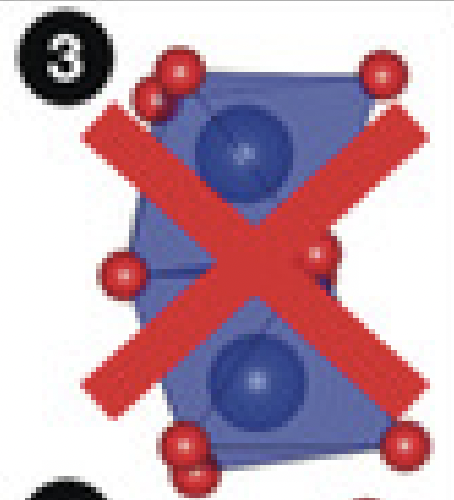
\includegraphics[height=1in]{Silde_Template/images/3.png}
    
    \begin{itemize}
        \item The decrease in stability is the result that sharing edges and faces places cations in closer proximity to each other, so that cation-cation electrostatic repulsion is increased.  \pause
        \item The effect is largest for cations with high charge and low C.N. (especially when $\frac{r_c}{r_a}$ approaches the lower limit of the polyhedral stability).
    \end{itemize}
\end{frame}

\begin{frame}{Pauling's Rule 3:  Example \ce{TiO2}}
    
    Ti in an octahedron CN=6\\[12 pt]
    Rutile - most stable - Shares 2 edges with no faces\\
    Brookite - slightly lower stability - Shares 3 edges with no faces\\
    Anatase - lowest stability - Shares 4 edges with no faces.\\[2em]
    \centering
    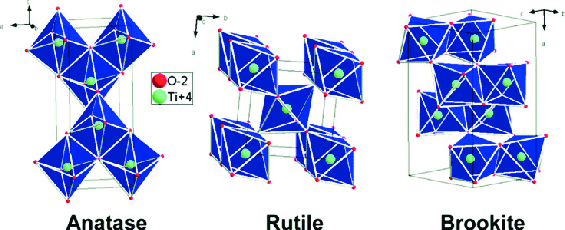
\includegraphics[height=1in]{Silde_Template/images/Rutile-anatase-and-brookite-unit-cells-all-showing-octahedral-titanium-coordination.png}
\end{frame}

 \begin{frame}{Pauling's Rule 4}

    \textbf{Rule 4:} Crystals containing different cations of high valence and a small CN tend not to share polyhedron elements with each other. \\[2em]
    
    \pause
    Example \ce{CaTiO3}:\\[0.5em]
     \ce{CaO12} polyhedra share edges \\
     \ce{TiO6} polyhedra share corners \\[1em] 
    
    \pause
    \justifying
    The \ce{Ti^{4+}} cation is more highly charged than the \ce{Ca^{2+}} cation, so the CN is smaller; the Coulombic repulsion between cations is proportional to the product of the charges.
    
 \end{frame}
 
\begin{frame}{Pauling's Rule 5}
\textbf{Rule 5:} The number of essentially different kinds of constituents in a crystal tends to be small\\[1em]
\pause

\centering
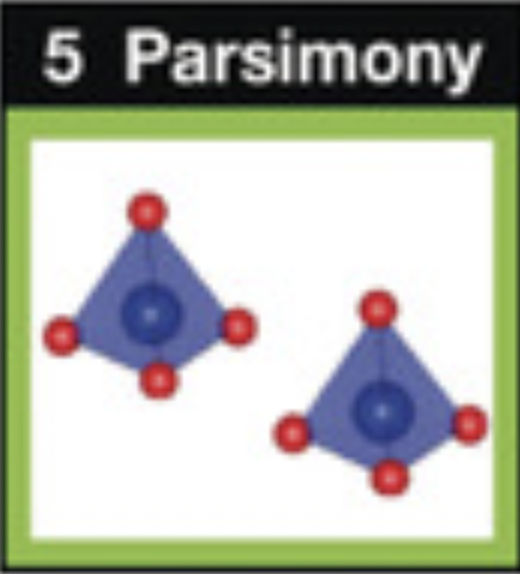
\includegraphics[height=1in]{Silde_Template/images/5.png}

\pause
\begin{itemize}
    \item As much as possible the environment of chemically similar atoms should be similar \pause
    \item This applies mostly to the coordination number (CN) \pause
    \item There is not a requirement that the structures are geometrically identical or indistinguishable.
\end{itemize}
\end{frame}

\begin{frame}{Summary of Rules}
\begin{enumerate}
    \item \textbf{Rule 1:} A coordinated polyhedron of anions is formed about each cation. The cation–anion distance is determined by the sum of the two radii, and the CN is determined by the radius ratio \pause
    \item \textbf{Rule 2:} In a stable structure, the total electrostatic strength of the bonds, S, reaching an anion in a coordination polyhedron from all neighboring cations should be equal to the charge of the anion \pause
    \item \textbf{Rule 3:} Polyhedra in a structure prefer not to share edges or faces. Clearly, if the faces are shared, at least three edges are also shared \pause
    \item \textbf{Rule 4:} Crystals containing different cations of high valence and a small CN tend not to share polyhedron elements with each other \pause
    \item \textbf{Rule 5:} The number of essentially different kinds of constituents in a crystal tends to be small
\end{enumerate}
    
\end{frame}

\section{Binary Crystal Structures}
\begin{frame}{Binary Ceramic Crystal Structures: Preface}
\begin{itemize}
    \item Crystal structures in ceramics are incredibly complex
    \pause
    \item We are going to introduce some of the most important ceramic crystal structure (some of which you might have seen before)
    \pause
    \item There are entire textbooks written on a single crystallographic structure or polymorphs of a single compound $\rightarrow$ We are going to cover this in part of a lecture
\end{itemize}
\end{frame}

\begin{frame}{Cesium Chloride - CsCl}
\begin{itemize}
    \item<1-> This is the simplest structure 
    \item<2-> Bravais lattice is simple cubic
    \item<3-> Two interpenetrating sc lattices, one of \ce{Cs^+} and one of \ce{Cl^-}. The two sublattices are displaced by 1/2<111>.
\end{itemize}

\centering
\includegraphics<1->[height=1in]{Silde_Template/images/CsCl.png}\\

\onslide<4->
\justifying
Using Pauling's Rules:\\
\centering
$r_{Cs^+}/r_{Cl^-} = 170/181 = 0.94$\\
\justifying
This is $>0.732$ thus the CN = 8\\


\begin{itemize}
    \item<5-> This structure does not appear to occur for oxides because the (divalent) cation radius would need to be >102.5 pm (\ce{O^{2-}} is 140 pm)
\end{itemize}
    
\end{frame}

\begin{frame}{Rock Salt - NaCl}
\begin{itemize}
    \item<1-> The NaCl (rock salt or halite) structure is quite simple.
    \item<2-> Found for sulfides and carbides and some oxides, including MgO, CaO, SrO, BaO, CdO, FeO, and NiO
    \item<3-> Two interpenetrating FCC lattices: one of anions and the other of cations displaced by 1/2<001> or by 1/2<111>.
    \item<4-> NaCl is not closed-packed $\rightarrow$ six nearest neighbors (CN is 6) so the packing of the anions must be less dense than fcc
\end{itemize}

\centering
\includegraphics<1->[height=1in]{Silde_Template/images/NaCl.png}\\

\onslide<5->
\justifying
Using Pauling's Rules:\\
\centering
$r_{Mg^+}/r_{O^-} = 0.6$\\
\justifying
This is $>0.414$ but $<0.732$ thus the CN = 6\\
    
\end{frame}

\begin{frame}{Zinc Blend - GaAs ($\beta$-SiC)}
\begin{itemize}
    \item<1-> This is the Zinc blend structure
    \item<2-> A very open crystallographic structure APF = 0.41
    \item<3-> Two interpenetrating FCC lattices: one of anions and the other of cations displaced by 1/4<111>
    \item<4-> Alternatively, you could consider this as an FCC lattice with 1/2 the tetrahedral sites occupied
\end{itemize}

\centering
\includegraphics<1->[height=1in]{Silde_Template/images/GaAs.png}\\
    
\end{frame}

\begin{frame}{Würzite AlN, BeO, ZnO}
\begin{itemize}
    \item<1-> HCP crystal structure with half of the tetragonal indexies with cations
    \item<2-> The CN is 4 for both the cations and the anions
\end{itemize}
    
\centering
\includegraphics<1->[height=1in]{Silde_Template/images/wurtzite.png}\\
    
\begin{itemize}
    \item<3-> BeO and AlN have both been used for electronic packaging because of their high thermal conductivity
    \item<4-> GaN is of great interest for manufacturing blue–green laser diodes and blue and green light-emitting diodes (LEDs)
\end{itemize}
\end{frame}

v\begin{frame}{\ce{CaF2}}

\centering
\includegraphics<1->[height=1in]{Silde_Template/images/florite.png}

\begin{itemize}
    \item<1-> arranging the \ce{Ca^{2+}} ions on an fcc lattice and then placing the \ce{F^{-}} anions on the 1/4,1/4,1/4 sites
    \item<2-> \ce{CaF2} is then the material of choice for semiconductor lithography. It is one of only a few materials that are transparent at the shorter wavelengths of deep-UV light
\end{itemize}

\onslide<3->
\justifying
Using Pauling's Rules:\\
\centering
$r_{Ca^{2+}}$ = 100 pm and $r_{F^{-}}$ = 130 pm
$r_{Ca^{2+}}$/$r_{F^{-}}$ = 0.8\\

\onslide<4->
\justifying
Thus the coordination number of $Ca^{2+}$ is 8, where ${F^{-}}$ is 4. \\
\onslide<5->
\emph{This is because of the charge}
\end{frame}

\begin{frame}{\ce{TiO2}}
    \begin{itemize}
        \item<1-> \ce{TiO2} exists as rutile, anatase, and brookite
        \item<2-> Each of these structures is different and it is more than just the packing
        \item<3-> \ce{Ti4+} cations in the center of oxygen octahedra
    \end{itemize}
\end{frame}

\begin{frame}{Rutile}
\begin{itemize}
    \item<1-> Has a tetragonal symmetry
    \item<2-> Structure is constructed by linking octahedra
    
    \centering
    \includegraphics<1->[height=1in]{Silde_Template/images/Rutile.png}
    
    \begin{itemize}
        \item<3-> An octahedron is placed at each of the eight corners such that two are actually sharing an apex (e.g., at T)
        \item<4-> The six points on these octahedra are then connected by one rotated octahedron sitting in the center of the unit cell
        \item<5-> Rutile is the most stable $\rightarrow$ recall from Pauling rules shares 2 edges
    \end{itemize}
    
\end{itemize}
\end{frame}

\begin{frame}{Brookite}

\centering
\includegraphics<1->[height=2in]{Silde_Template/images/Brookite.png}

\begin{itemize}
    \item<1-> Becomes orthorhombic in structure
    \item<2-> Each octahedron shares 3 of its edges
    \item<3-> Brookite is less stable than Rutile $\rightarrow$ shares 3 edges instead of 2
\end{itemize}
    
\end{frame}

\begin{frame}{Anatase}

\centering
\includegraphics<1->[height=2in]{Silde_Template/images/Anatase.png}

\begin{itemize}
    \item<1-> Still tetragonal but has a distorted octahedron
    \item<2-> Each octahedron shares 4 of its edges
    \item<3-> Anatase is less stable than Rutile or Brookite $\rightarrow$ shares 4 edges instead of 3 or 2
\end{itemize}
    
\end{frame}

\begin{frame}{\ce{Al2O3}}
\centering
\includegraphics<1->[height=2in]{Silde_Template/images/Aluminum.png}
\begin{itemize}
    \item<1-> Alumina refers to $\alpha$-\ce{Al2O3}
    \item<2-> Ruby $\rightarrow$ doped with \ce{Cr^{3+}} 
    \item<3-> Sapphire $\rightarrow$ doped with \ce{Ti^{3/4+}} and \ce{Fe^{2+}} 
\end{itemize}
    
\end{frame}

\begin{frame}{\ce{Al2O3}}
\centering
\includegraphics<1->[height=2in]{Silde_Template/images/Aluminum.png}
\begin{itemize}
    \item<2-> Actually has a $\bar{3}m$ symmetry but close to 6-fold so common to use hcp conventions
    \item<3-> Can be thought of as HCP for the oxygen with \ce{Al^{3+}} occupying 2/3 of the octahedral interstices ($P_1$ and $P_2$) are the missing octahedral
    \item<4-> To avoid sharing a face the the bond lengths distort
\end{itemize}
\end{frame}

\begin{frame}{\ce{Al2O3}}
\centering
\includegraphics<1->[height=2in]{Silde_Template/images/Al_faces.png}
\begin{itemize}
    \item<1-> There are common names for the different crystallographic faces in \ce{Al2O3}
    \item<2-> The properties are highly directional dependent
\end{itemize}
\end{frame}

\begin{frame}{\ce{MoS2}}

\centering
\includegraphics<1->[height=1.75in]{Silde_Template/images/MoS2.png}

\begin{itemize}
    \item<1-> Mo atoms are located in hcp structure 
    \item<2-> An S–S pair is centered along the c-direction directly opposite the Mo atoms
    \item<3-> Similar structure to graphite w/ weak van der Waals bonds between the planes
    \item<4-> Various stacking configurations because of the weak bonds
    \item<5-> Makes an excellent dry lubricant
\end{itemize}
    
\end{frame}

\section{Ternary Crystal Structures}
\begin{frame}{Spinel}

    \centering
    \includegraphics<1->[height=1.75in]{Silde_Template/images/Spinel.png}
    
    \begin{itemize}
        \item<1-> General formula \ce{AB2O4}
        \item<2-> Important because the magnetic ferrites are spinels
        \item<3-> The Bravais lattice is fcc, and the unit cell contains a total of 56 ions (32 oxygen ions).
        \item<4-> \ce{O^{2-}} ions as sitting on FCC lattice sites, A-site cation in some of tetragonal sites, and B-site cation on some of the octahedral sites
        
    \end{itemize}
\end{frame}

\begin{frame}{Spinel}
    \centering
    \includegraphics<1->[height=1.75in]{Silde_Template/images/Spinel.png}

\begin{itemize}
    \item<1-> \emph{Normal Spinel:} The \ce{A^{2+}} ions occupy only tetrahedral sites, and the \ce{B^{3+}} ions occupy only octahedral sites
    \item<2-> \emph{Inverse spinel:} All the \ce{A^{2+}} ions and half the \ce{B^{3+}} ions sit on the octahedral sites; the tetrahedral sites are occupied now by the other half of the \ce{B^{3+}} ions.
\end{itemize}    

\end{frame}

\begin{frame}{Visualizing Spinels}

\centering
\includegraphics<1->[height=1.6in]{Silde_Template/images/spinel_structure.png}


\begin{itemize}
    \item<1-> We can start by looking along the [110] $\rightarrow$ this is the closed-packed Oxygen plane.
    \item<2-> This sequence is PqRsTuVw, where the upper case refers to mixed \ce{O^{2-}} plus octahedral cation layers, and the lower case refers to the tetrahedral cations.
    \item<3-> You might ask how did they ever figure out this crystal structure \pause $\rightarrow$ They used structure factor and X-ray diffraction!
\end{itemize}
    
\end{frame}

\begin{frame}{Perovskite}
\begin{columns}{\textwidth}
  \begin{column}{0.33\textwidth}
  \centering
  \includegraphics<1->[height=2.5in]{Silde_Template/images/Perovskite.png}
  \end{column}
  \begin{column}{0.66\textwidth}
      \begin{itemize}
          \item<1-> \ce{ABO3},the A cation and the anions effectively form an FCC array with a large octahedron in the center
          \item<2-> Ideal, high-temperature structure is simple cubic $\rightarrow$ can undergo tetrahedral, monoclinic, and rhombohedral distortions
          \item<3-> Larger 2+ cations at the corners, smaller 4+ cation in the octahedral sites
          \item<4-> We will talk about Perovskites w/ ferroelectrics most good ferroelectrics are Peroskites
      \end{itemize}
  \end{column}
  \end{columns}
    
\end{frame}

\section{Important Concepts to Master}
\begin{frame}{Important Concepts to Master}
\begin{itemize}
    \item How to calculate ionic character of a bond
    \pause
    \item Definition of a Bravais Lattice
    \pause
    \item How to determine simple bonding configuration from constituent atoms with support of equations and tables
    \pause
    \item How to determine relative stability of different crystallographic structure in common materials (e.g., \ce{TiO2})
    \pause
    \item Given a crystallographic structure be able to predict some of the properties determined by the crystallographic structure
    \pause
    \item How coordination number relates to bonding and structural configuration (e.g. CN = 6, octahedral)
    \pause
    \item Be able to relate atomic radius and formal charge to bonding configuration
    \pause
\end{itemize}

Things you should not attend to:
\begin{itemize}
    \item Names of specific crystallographic structures
    \item Chemical composition of specific crystallographic structures
    \item The structure and drawings of specific crystallographic structures
\end{itemize}
    
\end{frame}
 
    





    


% \begin{frame}{Metals}

% \begin{itemize}
%     \item Constructed of atoms held together by delocalized electrons
%     \pause
%     \item They are commonly found as alloys with metallic and non-metallic elements
%     \pause
%     \item Delocalized electrons give metallic properties (e.g., good thermal and electrical conductivity)
%     \pause
%     \item Metallic bonding allows for closed-packed crystal structures that permit plastic deformation
% \end{itemize}
    
% \end{frame}

% \begin{frame}{Polymers}
% \begin{itemize}
%     \item Macromolecules formed by covalent bonding of many simpler molecular units called mers 
%     \pause
%     \item Most polymers are organic compounds based on carbon, hydrogen, and other nonmetals such as sulfur and chlorine 
%     \pause
%     \item The bonding between the molecular chains determines many of their properties
%     \pause
%     \item Many of the plastics that we are familiar with are actually combinations of polymers and often include fillers and other additives to give the desired properties and appearance
% \end{itemize}
% \end{frame}

% \begin{frame}{Ceramics}
% What are ceramics? 
% \pause
% \vspace{1em}

% \begin{itemize}
%     \item “mixed” bonding a combination of covalent, ionic, and sometimes metallic
%     \pause
%     \item They consist of arrays of interconnected atoms; there are no discrete molecules
%     \item The majority of ceramics are compounds of metals or metalloids and nonmetals
%     \pause
%     \item Most frequently they are oxides, nitrides, and carbides, however, diamond and graphite are considered ceramics.
% \end{itemize}
% \pause

% \vspace{1em}
% \textbf{Most solid materials that are not metal, plastic, or derived from plants or animals are ceramics}

% \end{frame}

% \begin{frame}{Semiconductors}

% \begin{itemize}
%     \item Only class of material based on a property
%     \pause
%     \item They are usually defined as having electrical conductivity between that of a good conductor and an insulator
%     \pause
%     \item The conductivity is strongly dependent upon the presence of small amounts of impurities
%     \pause
%     \item Classically, semiconductors have been limited to materials with a band gap $<3eV$, but there is growing commercial interest in large band gap semiconductors for high-temperature electronics.
% \end{itemize}
    
% \end{frame}

% \begin{frame}{Composites}
%     \begin{itemize}
%         \item Composites are materials formed by more than one material (sometimes this is extended to phase)
%         \pause
%         \item Usually there is a matrix and a filler
%         \pause
%         \item it is quite common to have ceramic composites
%     \end{itemize}
%         \pause
%         \centering
%         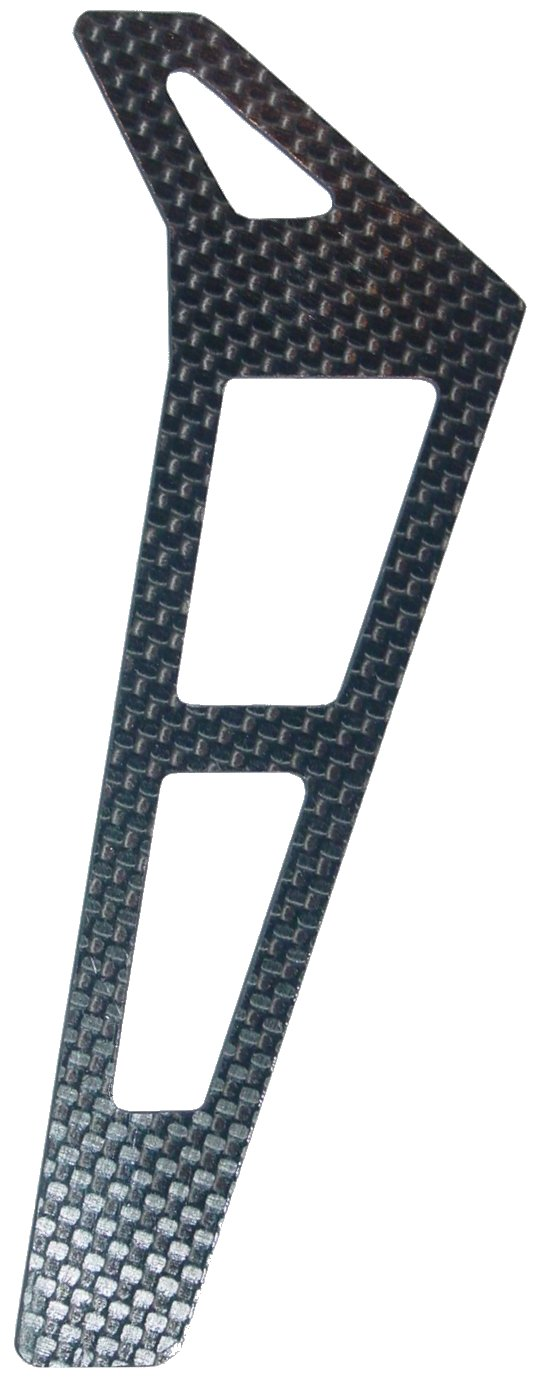
\includegraphics[height=1in]{Silde_Template/images/carbon_fiber.jpeg}
    
    
% \end{frame}

% \begin{frame}{Ceramic Ontologies and Exceptions}
% Exclusionary definition: Ceramic materials are inorganic, non-metallic solids.
% \pause

% \begin{itemize}
%     \item All inorganic semiconductors are ceramics
%     \pause
%     \item A materials ceases to be a ceramic when melted
%     \pause
%     \item All high-temperature superconductors are ceramics
%     \pause
%     \item Ice even though it is an inorganic material in the solid phase is not a ceramic
%     \pause
%     \item Glasses live in a gray area - it is really a supercooled liquid
% \end{itemize}
    
% \end{frame}

% \begin{frame}{Ceramic Ontologies and Exceptions}
% Ceramics cannot be defined based on their properties

% \begin{itemize}
%     \item We can’t say “ceramics are brittle” because some can be superplastically deformed and some metals can be more brittle: a rubber hose or banana at 77 K shatters under a hammer
%     \pause
%     \item We can’t say “ceramics are insulators” unless we put a value on the band gap (Eg) where a material is not a semiconductor.
%     \pause
%     \item We can’t say “ceramics are poor conductors of heat” because diamond has the highest thermal conductivity of any known material. Porous ceramics have some of the lowest thermal conductivity of any known materials.
% \end{itemize}
    
% \end{frame}

% \section{Properties of Ceramics}

% \begin{frame}{Brittleness}
%     \centering
%     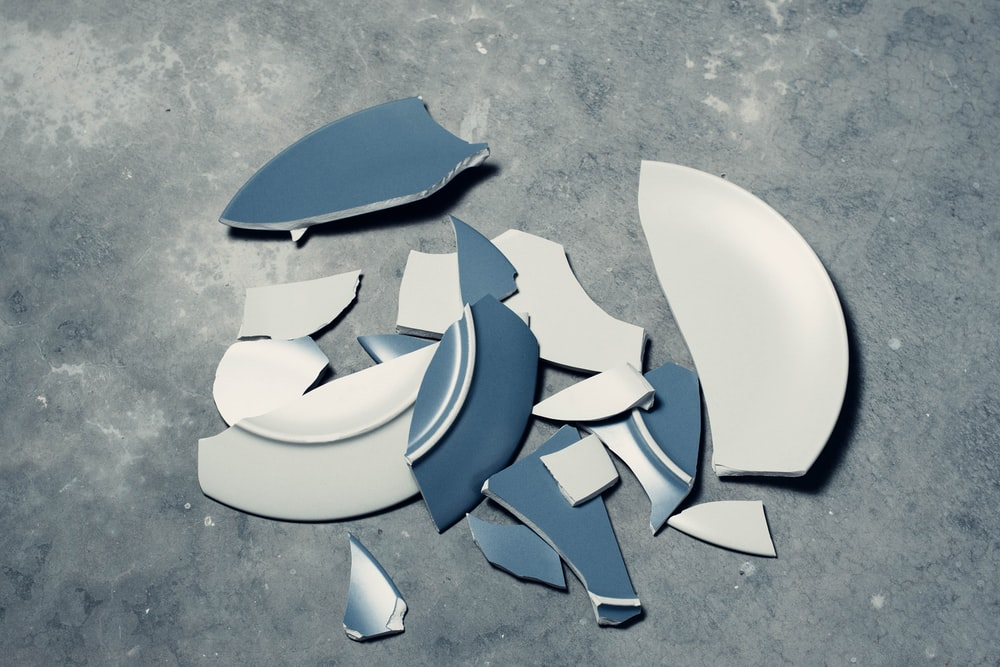
\includegraphics[height=1in]{Silde_Template/images/plate.jpeg}
    
%     \begin{itemize}
%         \item This property is recognized from personal experience, such as dropping a glass beaker or a dinner plate
%         \pause
%         \item The reason that the majority of ceramics are brittle is the mixed ionic-covalent bonding that holds the constituent atoms together
%         \pause
%         \item most ceramics are brittle at room temperature but not necessarily at elevated temperatures -- they can become viscous
%     \end{itemize}
    
% \end{frame}

% \begin{frame}{Poor electrical and thermal conduction}
    
%     \begin{itemize}
%         \item The valence electrons are tied up in bonds and are not free as they are in metals
%         \pause
%         \item Diamond, which we classified as a ceramic, has the highest thermal conductivity of any known material. \pause The conduction mechanism is due to phonons, not electrons.
%         \pause
%         \item The oxide ceramic $ReO_{3}$ has an electrical conductivity at room temperature similar to that of Cu
%         \pause
%         \item The mixed oxide $YBa_{2}Cu_{3}O_{7}$ is an HTSC; it has zero resistivity below 92 K
%     \end{itemize}
    
% \end{frame}

% \begin{frame}{Compressive Strength}
%     \centering
%     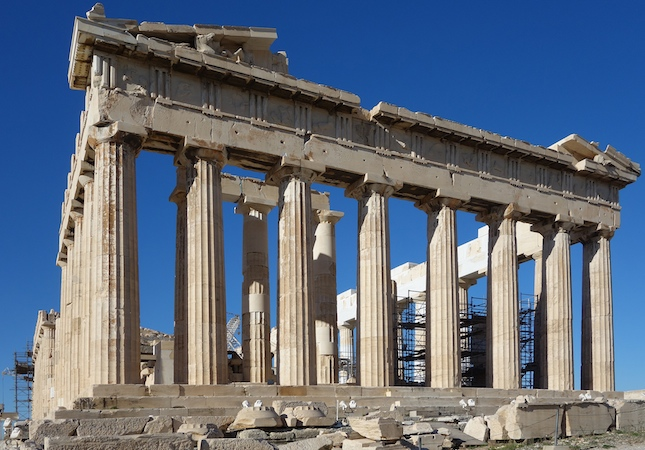
\includegraphics[height=1in]{Silde_Template/images/Greekcolumns.jpeg}
    
%     \begin{itemize}
%         \item Ceramics are stronger in compression than in tension, whereas metals have comparable tensile and compressive strengths \pause
%         \item This difference is important when we use ceramic components for load-bearing applications \pause
%         \item Ceramics generally have a low degree of toughness, although combining them in composites can dramatically improve this property
%     \end{itemize}
% \end{frame}

% \begin{frame}{Chemical insensitivity}

% \centering
% 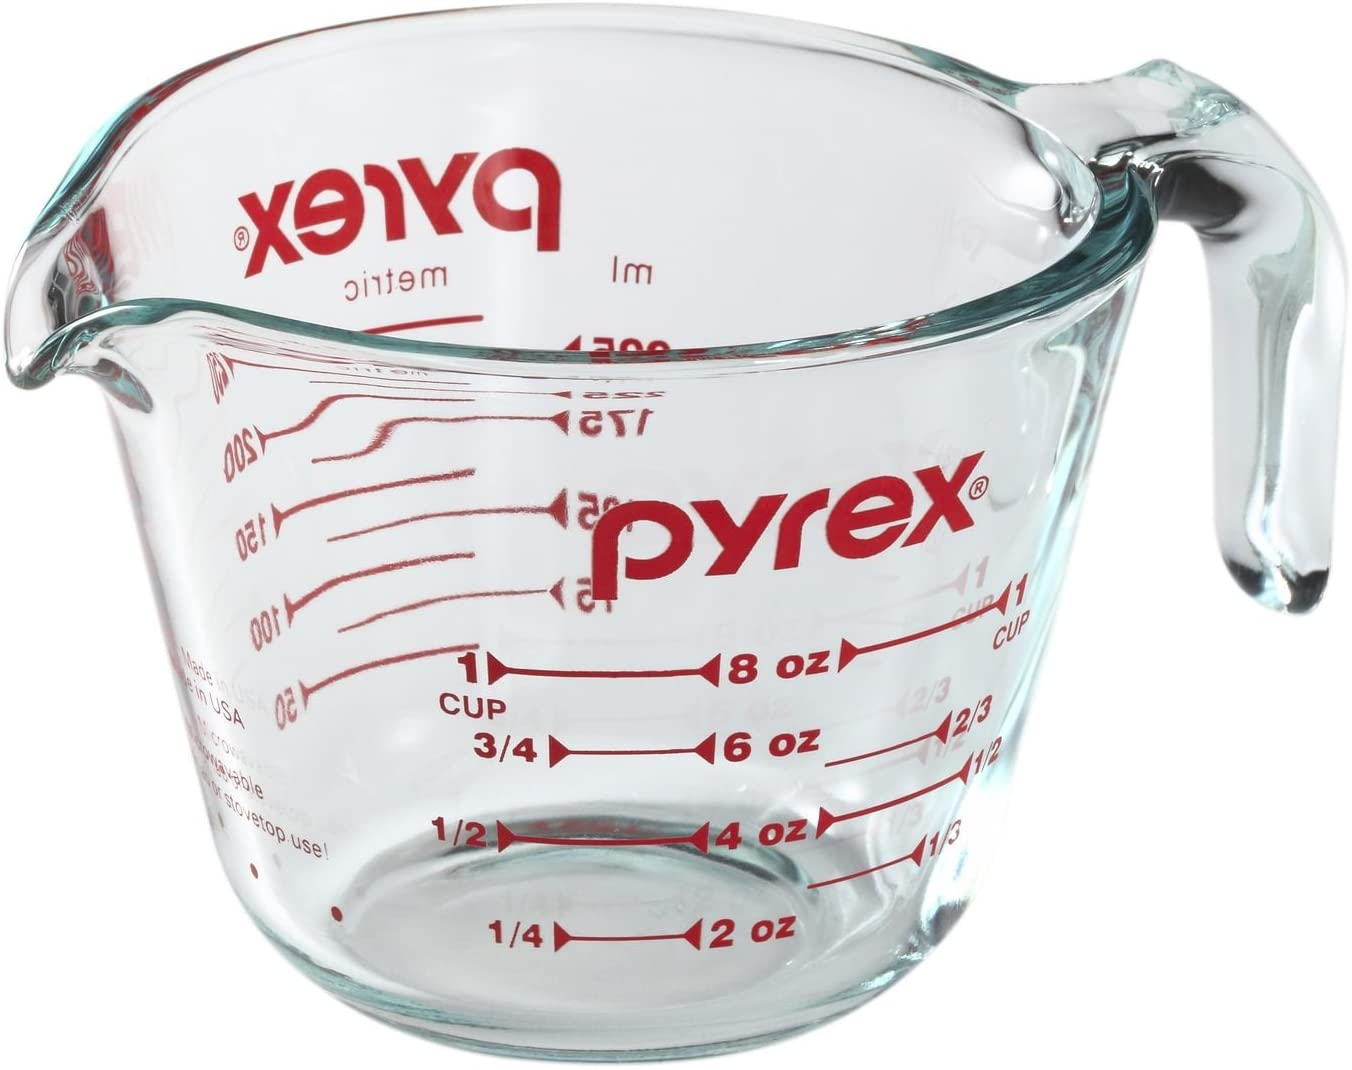
\includegraphics[height=1in]{Silde_Template/images/pyrex.jpg}

% \begin{itemize}
%     \item A large number of ceramics are stable in both harsh chemical and thermal environments
%     \pause
%     \item Example Pyrex: resistant to many corrosive chemicals, \pause stable at high temperatures (does not soften until 1,100 K),\pause and resistant to thermal shock because of its low coefficient of thermal expansion ($33x10^{-7} K^{-1}$)
% \end{itemize}
    
% \end{frame}

% \begin{frame}{Transparent}

% \centering
% 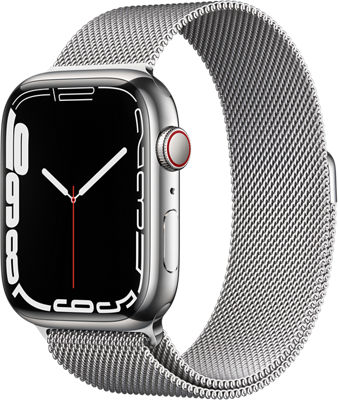
\includegraphics[height=1in]{Silde_Template/images/apple-watch-series-7-lte-45mm-silver-stainless-steel-silver-milanese-loop-mkje3ll-a-sku4790177.jpeg}

% \begin{itemize}
%     \item Many ceramics are transparent because they have a large $E_g$
%     \pause
%     \item Examples include sapphire watch covers, precious stones, and optical fibers.
%     \pause
%     \item Glass optical fibers have percent transmission > 96\%/km
%     \pause
%     \item "Clearly" not all ceramics are transparent
% \end{itemize}
    
% \end{frame}

% \begin{frame}{Traditional Ceramics}

% High volume items such as bricks, tiles, toilet bowls (whitewares), and pottery
% \vspace{1em}

% \begin{columns}{\textwidth}
%   \begin{column}{0.33\textwidth}
%     \centering
%     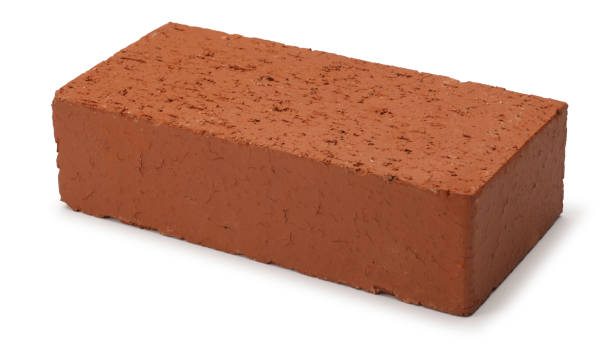
\includegraphics[height=1in]{Silde_Template/images/brick.jpeg}
%   \end{column}
%   \begin{column}{0.33\textwidth}
%   \centering
%     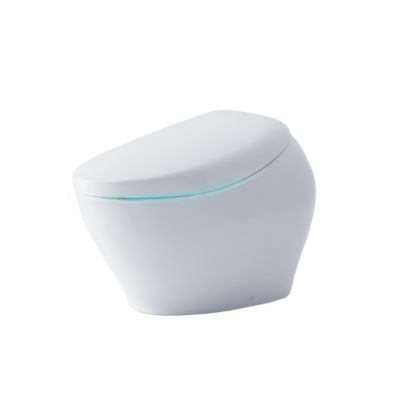
\includegraphics[height=1in]{Silde_Template/images/toilet.jpeg}
%   \end{column}
%     \begin{column}{0.33\textwidth}
%     \centering
%     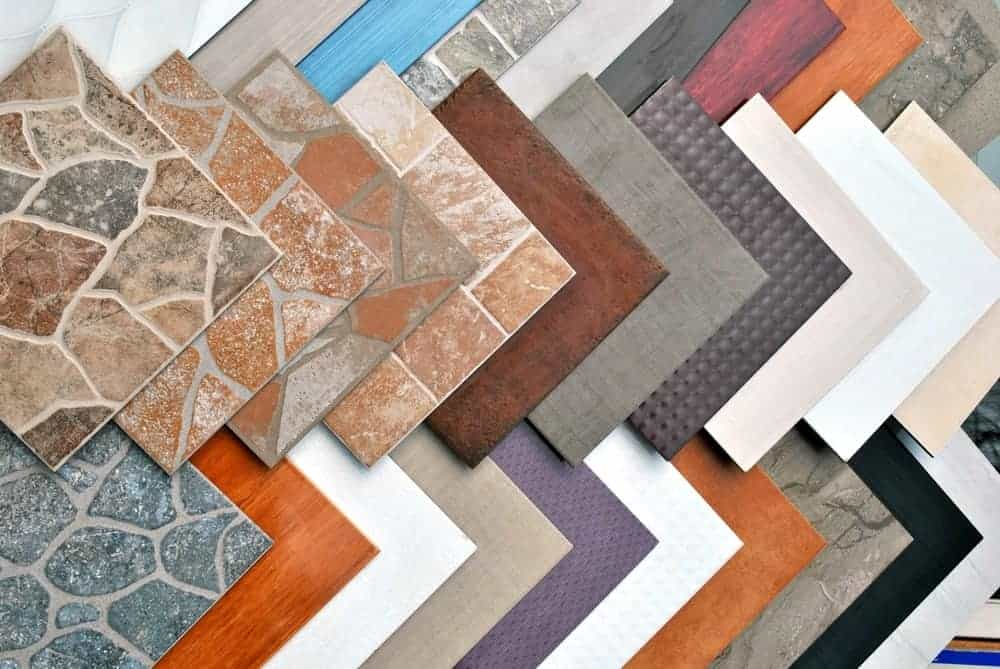
\includegraphics[height=1in]{Silde_Template/images/tiles.jpeg}
%   \end{column}
% \end{columns}
% \pause
% \begin{itemize}
%     \item Generally based on clay or silica
%     \item can require complex processing or tooling
% \end{itemize}
% \end{frame}

% \begin{frame}{Advanced or Technical Ceramics}

% \textbf{Advanced Ceramics}
% Advanced ceramics are newer materials, such as laser host materials, piezoelectric ceramics, and ceramics
% for dynamic random access memories (DRAMs), among others, which are often produced in small quantities at higher prices.    
% \vspace{1em}

% \begin{columns}
%   \begin{column}{0.33\textwidth}
%     \centering
%     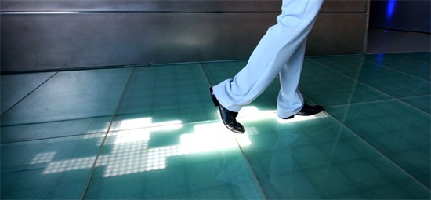
\includegraphics[height=1in]{Silde_Template/images/piezoelectric_floor.png}
%   \end{column}
%   \begin{column}{0.33\textwidth}
%     \centering
%     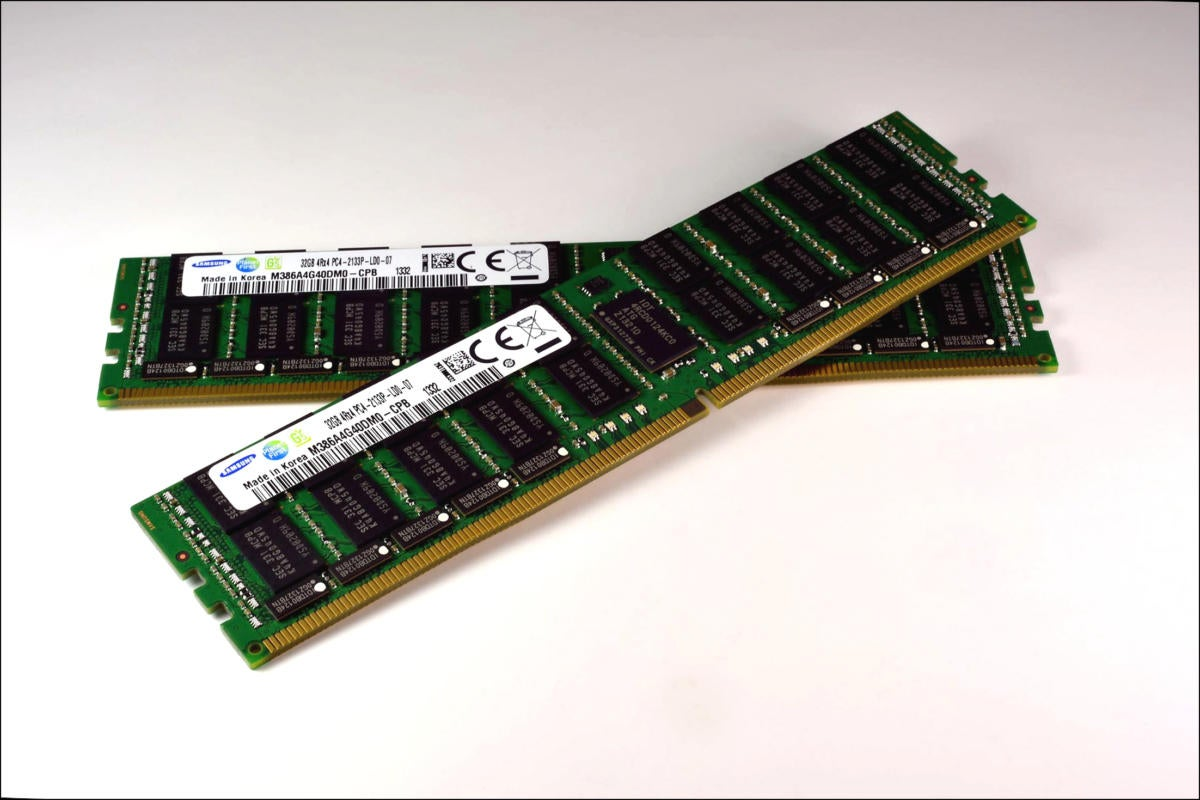
\includegraphics[height=1in]{Silde_Template/images/DRAM.jpeg}
%   \end{column}
%     \begin{column}{0.33\textwidth}
%     \centering
%     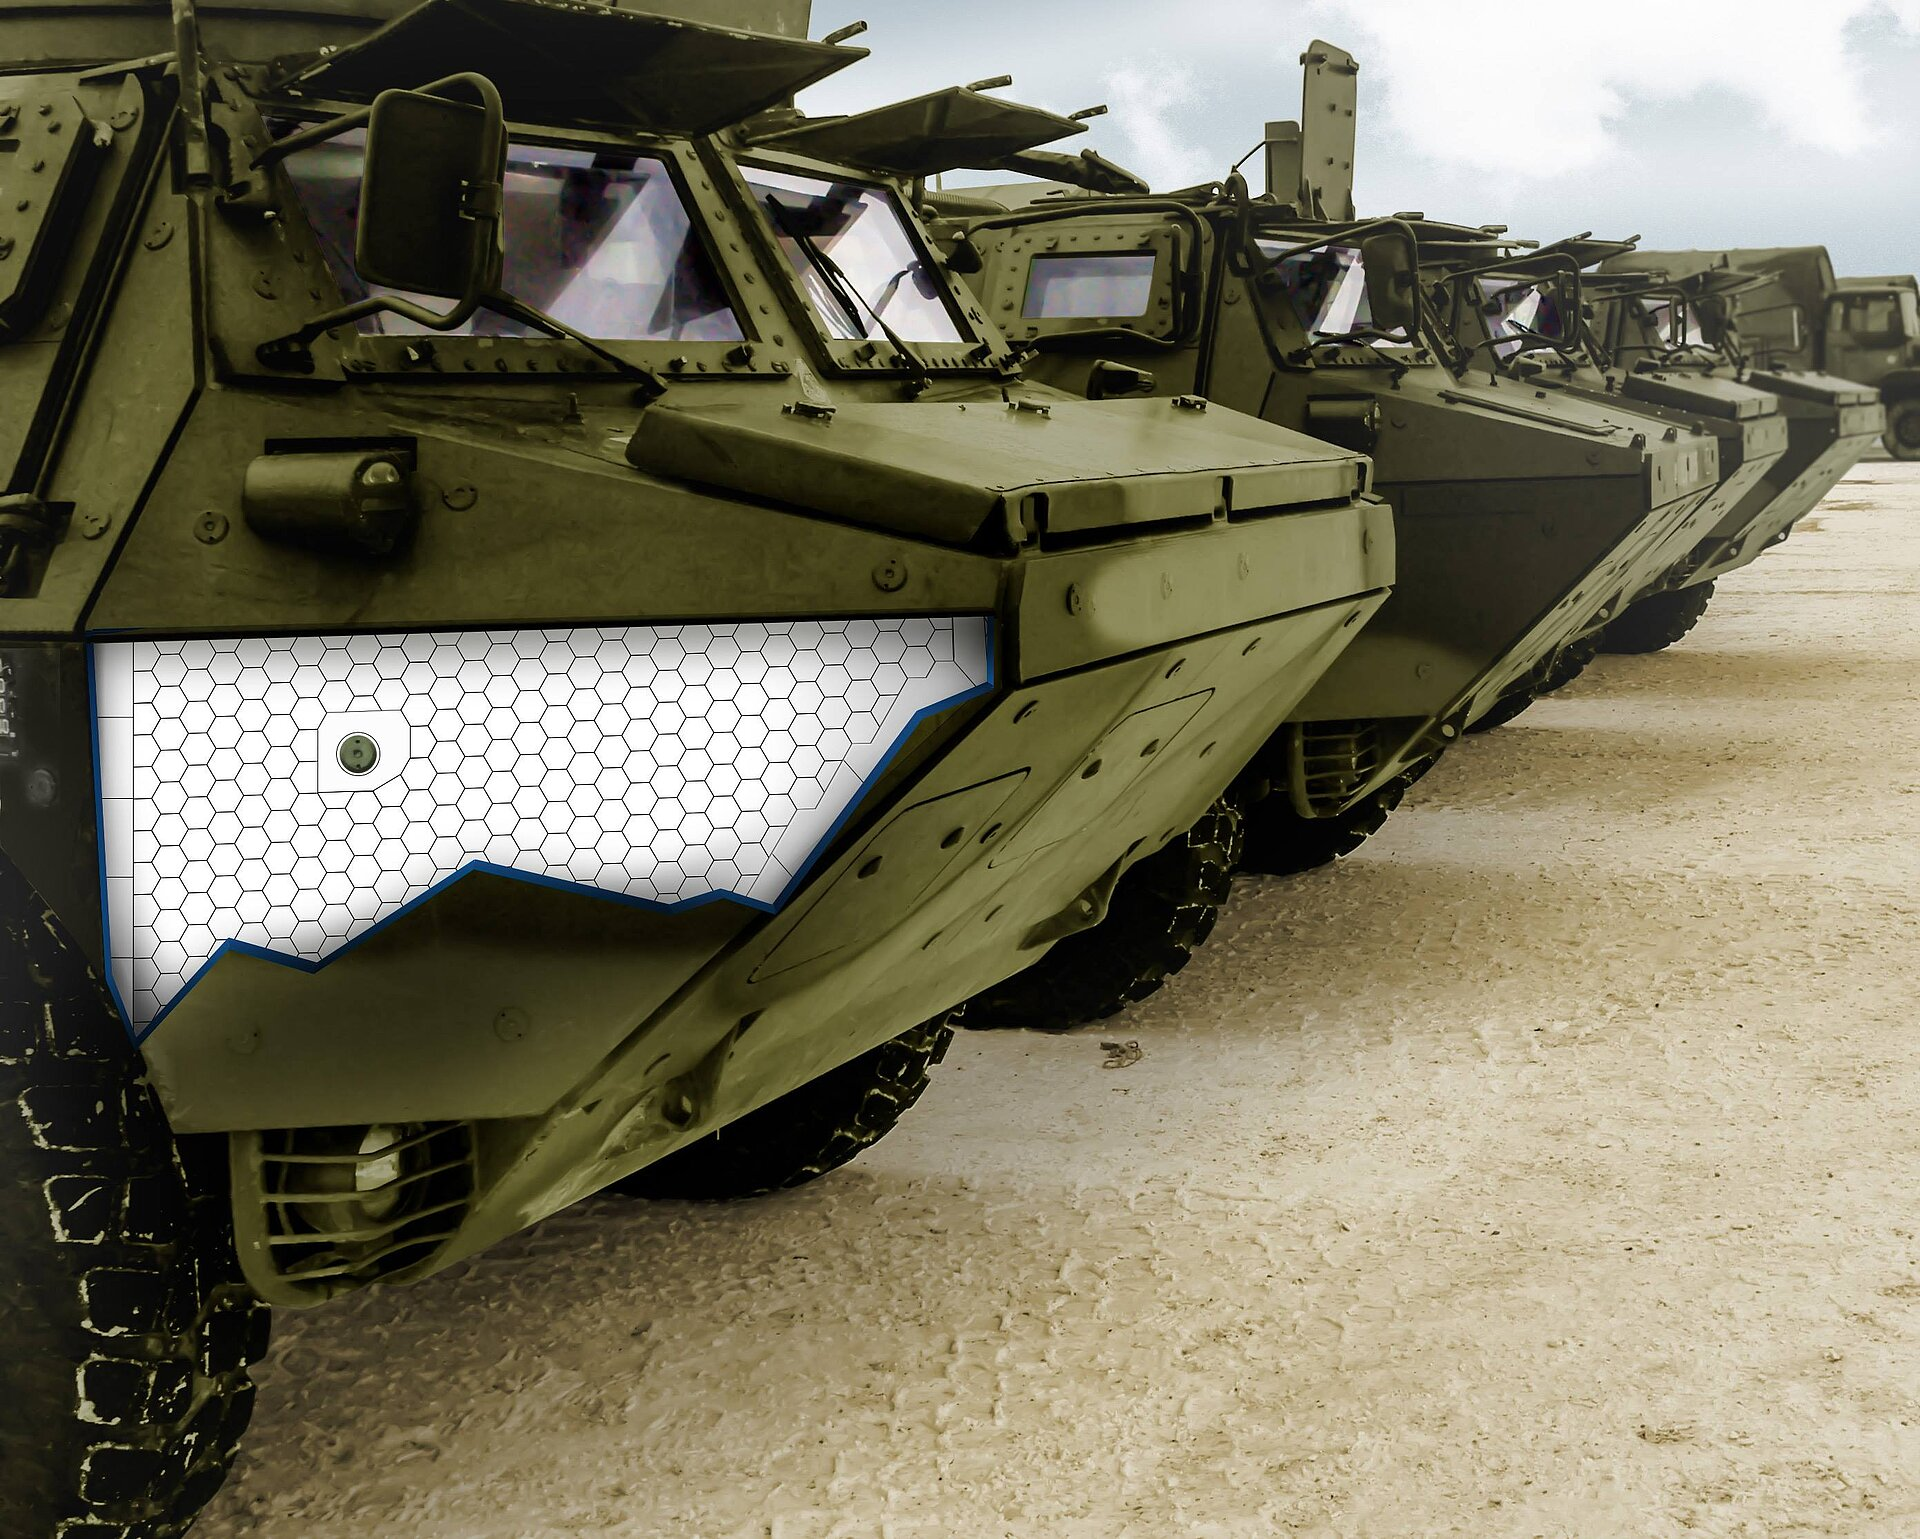
\includegraphics[height=1in]{Silde_Template/images/ballistic ceramics.jpeg}
%   \end{column}
% \end{columns}
% \pause
% \vspace{1em}

% \begin{itemize}
%     \item They exhibit superior mechanical properties, corrosion/oxidation resistance, or electrical, optical and/or magnetic properties.
%     \item Emerged primarily over the last 100 years
% \end{itemize}

% \end{frame}

% \begin{frame}{Properties and Applications of Ceramics}
% \centering
% 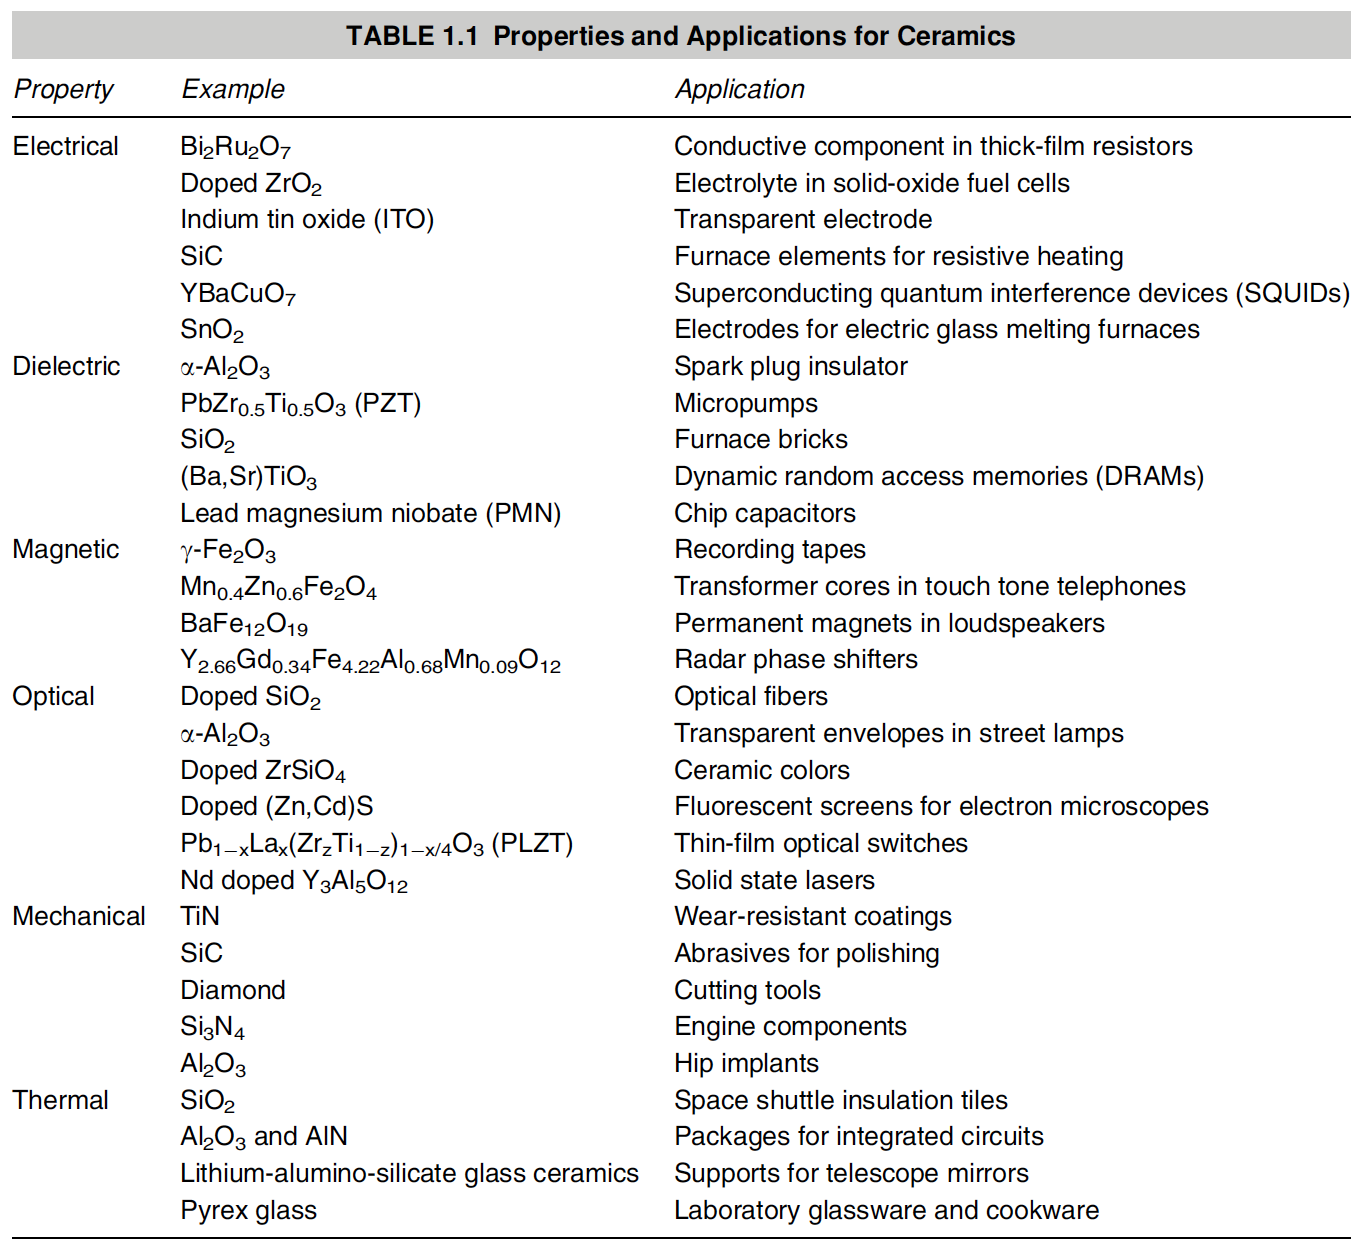
\includegraphics[height=\textheight]{Silde_Template/images/Properties of ceramics.png}
% \end{frame}

% \begin{frame}{Advanced vs. Traditional Ceramics}
% \centering
% 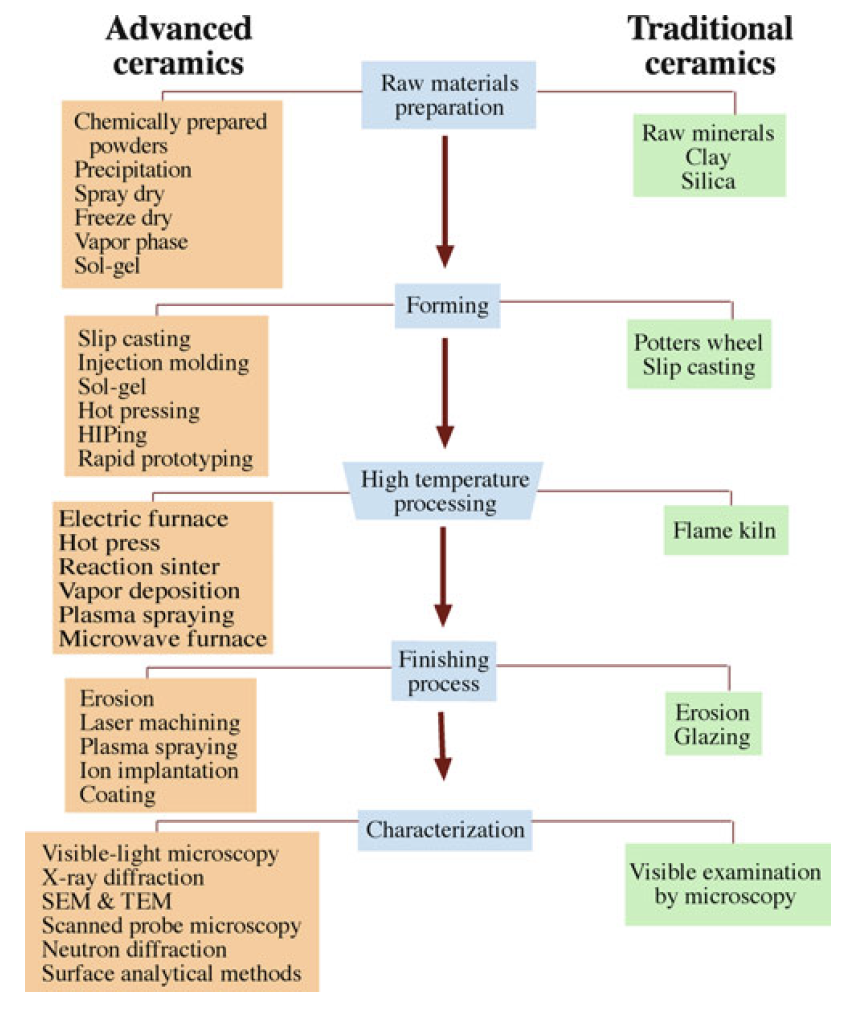
\includegraphics[height=\textheight]{Silde_Template/images/Comparison.png}
% \end{frame}

% \section{Market and Future}

% \begin{frame}{Overall Market Finances}
% Ceramics is a multibillion-dollar industry. Worldwide sales are about \$100 billion per year; the U.S. market alone is over \$35 billion annually.
% \vspace{1em}

% \centering
% 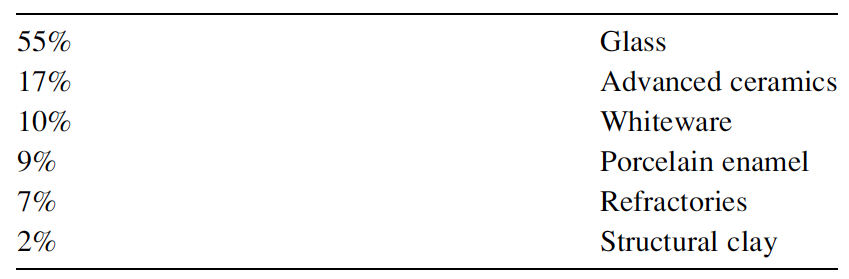
\includegraphics[width=0.75\textwidth]{Silde_Template/images/general market.png}
% \vspace{1em}

% \begin{itemize}
%     \item Bricks and glass, the commodity ceramics have the largest market
% \end{itemize}
    
% \end{frame}

% \begin{frame}{Advanced Ceramics}
% \vspace{1em}

% \centering
% 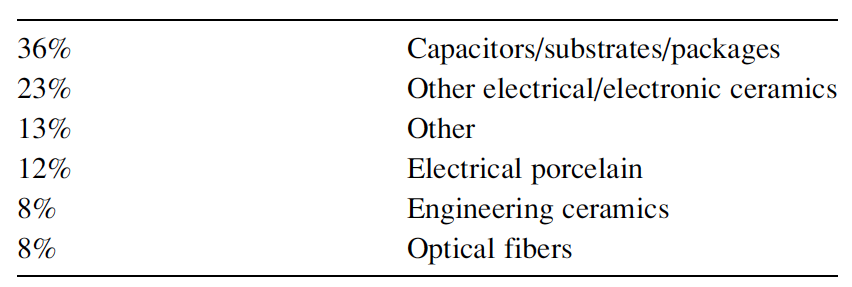
\includegraphics[width=0.6\textwidth]{Silde_Template/images/advanced ceramics.png}

% \begin{itemize}
%     \small
%     \item More than half of this sector is comprised of electrical and electronic ceramics and ceramic packages \pause
%     \item Significant growth areas include microwave filters and resonators for use in wireless communication \pause
%     \item Engineering ceramics, also called structural ceramics, include wear-resistant components such as dies, nozzles,and bearings\pause
%     \item Bioceramics (e.g., ceramic and glass-ceramic implants and dental crowns) account for about 20\% of this market (dental crowns) \pause 
%     \item Porcelain enamel is the ceramic coating applied to many steel appliances such as kitchen stoves, washers and dryers \pause
%     \item More than 50\% of refractories are consumed by the steel industry \pause
% \end{itemize}
% \end{frame}

% \begin{frame}{Structural Ceramics}
% \begin{itemize}
%     \item Include silicon nitride ($Si_3N_4$), silicon carbide ($SiC$), zirconia ($ZrO_2$), boron carbide ($B_4C$), and alumina ($Al_2O_3$)
%     \pause
%     \item They are used in applications such as cutting tools, wear components, heat exchangers, and engine parts
%     \pause
%     \item The relevant properties of structural ceramics are high hardness, low density, high-temperature mechanical strength, creep resistance, corrosion resistance, and chemical inertness
%     \pause
% \end{itemize}
% \vspace{1em}

% \textbf{Key Issues}
% \begin{itemize}
%     \item Reducing the cost of the final product
%     \item Improving reliability
%     \item Improving reproducibility
% \end{itemize}

% \end{frame}

% \begin{frame}{Electrical Ceramics}
% \begin{itemize}
%     \item Include barium titanate ($BaTiO_3$), zinc oxide ($ZnO$), lead zirconate titanate [$Pb(Zr_xTi_{1-x})O_3$], aluminum nitride ($AlN$), and high-temperature superconductors \pause
%     \item They are used in applications as diverse as capacitor dielectrics, varistors, micro-electro-mechanical systems (MEMS), substrates, and packages for integrated circuits \pause
% \end{itemize}

% \textbf{Key Issues}
% \begin{itemize}
%     \item Integrating with existing semiconductor technology
%     \item Improving processing
%     \item Enhancing compatibility with other materials
%     \item Improved electrical resistivity in thin films
% \end{itemize}

% \end{frame}

% \begin{frame}{Bioceramics}
% \begin{itemize}
%     \item The response of these materials varies from nearly inert to bioactive to resorbable \pause
%     \item Nearly inert bioceramics include alumina ($Al_2O_3$) and zirconia ($ZrO_2$) \pause
%     \item Bioactive ceramics include hydroxyapatite and some special glass and glass-ceramic formulations \pause
%     \item Tricalcium phosphate, which dissolves in the body, is an example of a resorbable bioceramic \pause
% \end{itemize}

% \textbf{Key Issues}
% \begin{itemize}
%     \item Matching mechanical properties to human tissues
%     \item Increasing reliability
%     \item Enhancing compatibility with other materials
%     \item Improving processing methods
% \end{itemize}
    
% \end{frame}

% \begin{frame}{Coating and Films}
%     \begin{itemize}
%         \item Coatings and films are generally used to modify the surface properties of a material (e.g., a bioactive coating deposited on the surface of a bio-inert implant) \pause
%         \item They may also be used for economic reasons: we may want to apply a coating of an expensive material on a lower cost substrate rather than make the component entirely from the more expensive material \pause $\rightarrow$ An example is applying a diamond coating on a cutting tool \pause
%         \item Thin film properties can be better, the transport properties of thin films of HTSCs, which are improved over the bulk
%     \end{itemize}


% \textbf{Key Issues}
% \begin{itemize}
%     \item Understanding film deposition and growth
%     \item Improving film/substrate adhesion
%     \item Increasing reproducibility
% \end{itemize}

% \end{frame}
% \begin{itemize}
%     \item Composites may use ceramics as the matrix phase and/or the reinforcing phase \pause
%     \item The purpose of a composite is to display a combination of the preferred characteristics of each of the components \pause
%     \item Ceramic matrix composites increase fracture toughness through reinforcement with whiskers or fibers \pause
%     \item Metal matrix composites usually an increase in strength, enhanced creep resistance, and greater wear resistance \pause
% \end{itemize}
% \begin{frame}{Composites}

% \textbf{Key Issues}
% \begin{itemize}
%     \item Reducing processing costs
%     \item Developing compatible combinations of materials (e.g., matching coefficients of thermal expansion)
%     \item Understanding interfaces
% \end{itemize}

% \end{frame}

% \begin{frame}{Nanoceramics}
% \begin{itemize}
%     \item Widely used in cosmetic products (e.g., sunscreens), as stabilizers, and they are critical in many catalytic applications \pause
%     \item Modern applications in quantum dots, fuel cells, and specialty coating applications \pause
% \end{itemize}

% \textbf{Key Issues}
% \begin{itemize}
%     \item Making them
%     \item Integrating them into devices through either top-down or bottom-up approaches
%     \item Ensuring that they do not have a negative impact on society
% \end{itemize}

% \end{frame}

\end{document}



        
